\documentclass{article}
\usepackage[fontsize=13pt]{fontsize}
\usepackage[utf8]{inputenc}
\usepackage[sfdefault]{roboto}
\usepackage[T1]{fontenc}
\usepackage[ngerman]{babel}
\usepackage{amsmath,amsfonts,amssymb,amstext,esdiff}
\usepackage{geometry}
\usepackage{parskip}
\usepackage{svg}
\usepackage{float}
\usepackage{afterpage}
\usepackage{listings}
\usepackage{pdfpages}
\usepackage{hyperref}
\usepackage{cleveref}
\usepackage{multirow}
\usepackage{xltabular}
\usepackage{wrapfig}
\usepackage{fancyhdr}
\usepackage{caption}
\usepackage[framemethod=default]{mdframed} % Required for comment environment
\usepackage{tikz}
\usepackage[automake,toc,section=section]{glossaries}
\newcommand{\OPT}[1]{{\color{teal} #1}}

\gdef\contentsname{Inhaltsverzeichnis}
\gdef\listfigurename{Abbildungsverzeichnis}
\gdef\listtablename{Tabellenverzeichnis}
%!TEX option = --shell-escape

\definecolor{dmGreen}{HTML}{009661}
\definecolor{htmlBlue}{HTML}{0060ff}

\definecolor{ocre}{RGB}{243,102,25}
\definecolor{codegreen}{rgb}{0,0.6,0}
\definecolor{codegray}{rgb}{0.5,0.5,0.5}
\definecolor{codepurple}{rgb}{0.58,0,0.82}
\definecolor{backcolour}{rgb}{0.95,0.95,0.92}
\lstdefinestyle{mystyle}{
commentstyle=\color{codegreen},
keywordstyle=\color{magenta},
numberstyle=\tiny\color{codegray},
stringstyle=\color{codepurple},
basicstyle=\ttfamily\footnotesize,
breakatwhitespace=false,
breaklines=true,
captionpos=b,
keepspaces=true,
numbers=left,
numbersep=5pt,
showspaces=false,
showstringspaces=false,
showtabs=false,
tabsize=2
}

\lstset{style=mystyle}
\geometry{
    a4paper,
    left=25mm,
    right=25mm,
    top=10mm,
    bottom=10mm,
    includeheadfoot,
    heightrounded
}

\newcommand{\argmin}[1]{\underset{#1}{\operatorname{argmin}}}
\newcommand{\para}[1]{\vspace{-5mm}\subsubsection*{#1}\vspace{-4mm}}

\renewcommand{\baselinestretch}{1.2}

% \renewcommand*{\arraystretch}{1.4}
\captionsetup[figure]{labelfont={bf},name={Figure}} % Caption title for figures/images
\captionsetup[table]{labelfont={bf},name={Table}}
\setlength{\belowcaptionskip}{-6pt} % reduce padding/mardin below figure and table captions

\hypersetup{
    colorlinks=true,
    anchorcolor=black,
    citecolor=htmlBlue, % citations
    linkcolor=htmlBlue, % in-document links
    filecolor=black,
    urlcolor=htmlBlue, % \href{URL}{text} usages
    pdftitle={D6_Lastenheft_Pong},
    pdfauthor={Leon Wiesen}
}

\setcounter{secnumdepth}{5}
\setcounter{tocdepth}{5}

\pagestyle{fancy}
\fancyhf{}
\lhead{\rightmark}
\rhead{Lastenheft PONG}
\cfoot{\thepage}

\makeglossaries
%Kommas werden am Ende jeder Definition automatisch hinzugefügt.

\newglossaryentry{muss}{ name={muss}, description={
    Diese Funktion ist verbindlich
}}
\newglossaryentry{sollte}{ name={sollte}, description={
    Diese Funktion ist optional und wird implentiert, wenn die notwendigen Ressourcen zur Verfügung stehen
}}
\newglossaryentry{balken}{ name=Balken, description={
    Das einzige Spielelement, welches der Spieler aktiv kontrollieren kann. Der horizontale Balken ist am unteren Bereich des Spielfelds positioniert und der Ball prallt von diesem ab
}}
\newglossaryentry{ball}{ name=Ball, description={
    Das zentrale Spielelement, welches vom Balken und von allen Rändern des Spielfelds abprallt und durch die physikalische
    Interaktion mit dem Balken indirekt vom Spieler gesteuert wird
}}
\newglossaryentry{beta}{name={Beta-Version},description={
    Eine vorläufige und funktionstüchtige Testversion des Spiels, die der Erhaltung von Feedback dient und diesem dynamisch angepasst wird
}}
\newglossaryentry{block}{ name=Block, description={
    Ein Spielobjekt, welches im Invasion-Mode vom Ball zerstört werden muss
}}
\newglossaryentry{classicMode}{ name=Classic-Mode, description={
    Der klassische PONG-Spielmodus, bei dem nur ein Ball und ein Balken auf dem Spielfeld existiert
}}
\newglossaryentry{coin}{ name=Coin, description={
    Die Währung des Spiels
}}
\newglossaryentry{invasionMode}{ name=Invasion-Mode, description={
    Ein erweiterter Spielmodus, bei dem der Ball zusätzlich Block-Objekte zerstört
}}
\newglossaryentry{ladezeiten}{ name=Ladezeiten, description={
    Die Wartezeit beim initialen Laden der App (Starten aus dem Betriebssystem) und Wechsel zwischen Menüs
}}
\newglossaryentry{leben}{ name=Leben, description={
    Eine abstrakte Währung, die der Beendigung eines Spieldurchlaufs dient. Besitzt der Spieler keine Leben mehr, endet das Spiel
}}
\newglossaryentry{niceToHave}{ name=Nice-To-Have, description={
    Optionale Anforderungen, die nicht rechtlich bindend und deren Implementierung völlig dem Entwicklerteam überlassen sind
}}
\newglossaryentry{powerup}{ name=Power-Up, description={
    Ein temporärer Effekt, der z.B. Spielelemente wie den Ball oder den Balken betrifft und deren Verhalten ändert
}}
\newglossaryentry{release}{name={Release-Version},description={
    Die finale und ausgelieferte Version des Spiels
}}
\newglossaryentry{tail}{ name=Schweif, description={
    Kosmetikeffekt hinter dem Ball, welcher die Bahnkurve anzeigt (gleicht dem Schweif einer Sternschnuppe)
}}
\newglossaryentry{point}{ name=Score-Point, description={
    Ein Wert, der dem Spieler als Metrik für seine Fähigkeiten dient. Im Verlauf des Spiels sammelt der Spieler zwangsläufig mehr
}}
\newglossaryentry{skin}{ name=Skin, description={
    Kosmetikeffekte wie verschiedene Sprites/Texturen für Ball, Balken und Spielhintergrund.
    Diese können im Store gegen Coins eingetauscht werden
}}
\newglossaryentry{spieler}{ name=Spieler, description={
    Jede Person, die die Anwendung nutzt \textit{Synonyme: Benutzer, Anwender}
}}
\newglossaryentry{spielfeld}{ name=Spielfeld, description={
    Umfasst den Bereich, in dem das Spiel stattfindet Vertikale Abgrenzungen sind der linke und rechte Bildschirmrand.
    Der obere Bildschirmrand bildet die obere Abgrenzung, die untere Abgrenzung erfolgt auf der Höhe, auf der sich der
    Balken befindet
}}
\newglossaryentry{Top10}{ name=Top-10, description={
    Die zehn besten Scores, die lokal auf einem Gerät (seit Installation) erreicht wurden
}}
\newglossaryentry{achievements}{ name=Achievements, description={
    Errungenschaft, die der Spieler im Laufe des Spiels freischalten kann, welche weder funktionelle noch kosmetische Auswirkungen auf das Spielgeschehen haben
}}
\newglossaryentry{kann}{ name=kann, description={
    Benennt eine optionale Anforderung (siehe "Nice-To-Have")
}}

\begin{document}
\setlength{\emergencystretch}{3em}  % fixes right-margin text overflows

\gdef\contentsname{Inhaltsverzeichnis}
\gdef\listfigurename{Abbildungsverzeichnis}
\gdef\listtablename{Tabellenverzeichnis}
    \pagenumbering{gobble}
    \selectlanguage{english}

    
\begin{titlepage} % Suppresses displaying the page number on the title page and the subsequent page counts as page 1
	\newcommand{\HRule}{\rule{\linewidth}{0.5mm}} % Defines a new command for horizontal lines, change thickness here
	
	\center % Centre everything on the page
	
	%------------------------------------------------
	%	Headings
	%------------------------------------------------
	
	\textsc{\LARGE Software Engineering WS22/23}\\[1.5cm] % Main heading such as the name of your university/college
	
	\textsc{\Large ISLCM Gruppe 8}\\[0.5cm] % Major heading such as course name
	
	\textsc{\large SWE Praktikumsgruppe D6}\\[0.5cm] % Minor heading such as course title
	
	%------------------------------------------------
	%	Title
	%------------------------------------------------
	
	\HRule\\[0.4cm]
	{\huge\bfseries Lastenheft: Mobile App PONG}\\[0cm] % Title of your document
	\HRule\\[0.4cm]
	
	%------------------------------------------------
	%	Author(s)
	%------------------------------------------------
	
    \begin{xltabular}{\linewidth}{l X r}
        \textbf{Projektmanagement} & & \textbf{Qualitätssicherung} \\
        Marc-André Hein         & & Dorian Ailin Hövelmann                  \\
        Felix Horn              & & Tobias Bogner               \\
        & & \\
        \textbf{Technologie}    & & \textbf{Vertrieb}           \\
        Markus Helm             & & Hristomir Dimov             \\
        Daniel-Michel Richter   & & Leon Wiesen                 \\
    \end{xltabular}
    \label{tab:table_of_members}
    
    
	% If you don't want a supervisor, uncomment the two lines below and comment the code above
	%{\large\textit{Author}}\\
	%John \textsc{Smith} % Your name
	
	%------------------------------------------------
	%	Date
	%------------------------------------------------
	
	\vfill\vfill\vfill % Position the date 3/4 down the remaining page
	
	\textbf{Version 2.1} \\
	\textit{09.11.2022} \\
	\vspace*{0.4cm}
	Vorgelegt von: \\
	Leon Wiesen
	%------------------------------------------------
	%	Logo
	%------------------------------------------------
	
	%\vfill\vfill
	%\includegraphics[width=0.2\textwidth]{placeholder.jpg}\\[1cm] % Include a department/university logo - this will require the graphicx package
	 
	%----------------------------------------------------------------------------------------
	
	\vfill % Push the date up 1/4 of the remaining page
	
\end{titlepage}


    \gdef\contentsname{Inhaltsverzeichnis}
    \tableofcontents
    \clearpage

    \section*{Changelog}\label{sec:changelog}
    \addcontentsline{toc}{section}{\protect\numberline{}Changelog}
    Die folgenden Änderungen wurden im Laufe der Entwicklung des Lastenhefts vollzogen. Diese erfolgten aus den Gesprächen und dem Schriftverkehr zwischen Kunden (siehe \hyperref[sec:auftraggeber]{Auftraggeber}) und dem Vertrieb (Hristomir Dimov \& Leon Wiesen).

\begin{xltabular}{\textwidth}{|c|X|}
    \hline
    \textbf{Version}   & \textbf{Änderungen}     \\
    \hline

    v0.0  \textit{(27.10.2022)} &  \begin{itemize}
        \item Kap. \ref{sec:funktionen}: Hinzugefügt
        \item Kap. \ref{sec:requirements}: Hinzugefügt
    \end{itemize}
    \\ \hline

    v0.1  \textit{(03.11.2022)} &  \begin{itemize}
        \item Kap. \ref{sec:auftraggeber}: Hinzugefügt
        \item Kap. \ref{sec:zeitbudget}: Hinzugefügt
        \item Kap. \ref{sec:bestimmung}: Hinzugefügt
        \item Kap. \ref{sec:einsatz}: Hinzugefügt
        \item Kap. \ref{sec:funktionen}: Neue MockUps
        \item Kap. \ref{sec:produktdaten}: Hinzugefügt
        \item Kap. \ref{sec:performance}: Hinzugefügt
        \item Kap. \ref{sec:quality}: Hinzugefügt
        \item Kap. \ref{sec:requirements}: Requirements erweitert
    \end{itemize}
    \\ \hline

    v1.0  \textit{(07.11.2022)} & \begin{itemize}
        \item Rechtscheib- \& Grammatikfehler korrigiert
        \item Glossar: Neue Begriffe Hinzugefügt
        \item Deckblatt: Gruppenname vervollständigt
        \item Deckblatt: Build-Datum hinzugefügt
        \item Kap. \ref{sec:auftraggeber}: Spezifischer formuliert
        \item Kap. \ref{sec:zeitbudget}: Glossar-Verlinkungen
        \item Kap. \ref{sec:zeitbudget}: Ausführlichere Grafik
        \item Kap. \ref{sec:einsatz}: Use-Case Diagramm hinzugefügt
        \item Kap. \ref{sec:funktionen}: Neue Diagramme
        \item Kap. \ref{sec:funktionen}: Genauere Beschreibungen
        \item Kap. \ref{sec:funktionen}: Glossar-Verlinkungen
        \item Kap. \ref{sec:produktdaten}: Genauere Beschreibungen
        \item Kap. \ref{subsec:lieferumfang}: Lieferumfang hinzugefügt
        \item Kap. \ref{sec:performance}: Minimierung auf das Nötigste
        \item Kap. \ref{sec:requirements}: Achievements sind jetzt mandatory (\gls{muss})
        \item Abnahme Hinzugefügt
    \end{itemize}
    \\ \hline

    v1.1  \textit{(08.11.2022)} & \begin{itemize}
        \item Rechtscheib- \& Grammatikfehler korrigiert
        \item Korrekte Verlinkung der Kapitel \& Bilder
        \item Vereinheitlichung von Begrifflichkeiten
        \item Vereinheitlichung von Begrifflichkeiten
        \item Glossar: Neue Begriffe Hinzugefügt
        \item Kap. \ref{sec:funktionen}: Korrekte Nummerierung der Bilder
        \item Kap. \ref{sec:funktionen}: Korrektur von Diagrammen
        \item Kap. \ref{subsec:balancing}: Hinzugefügt
    \end{itemize}
    \\ \hline

    v2.0  \textit{(09.11.2022)} & \begin{itemize}
        \item Rechtscheib- \& Grammatikfehler korrigiert
        \item Glossar: Einheitliche Benennung
        \item Glossar: Neue Begriffe hinzugefügt
        \item Zeitbudget vervollständigt
        \item Kap.~\ref{subsec:balancing}: Hinzugefügt
        \item Kap.~\ref{subsec:tests}: Hinzugefügt
        \item Hinweise vereinheitlicht
        \item Kap.~\ref{sec:funktionen}: Use-Case Diagramm angepasst
        \item Falsche automatische Silbentrennung korrigiert
        \item Figure-Benennung in Texten
        \item Figure~\ref{fig:dia:u40}: Platzhalter ausgetauscht gegen Werte
        \item Abnahme Auf \ref{subsec:balancing}, \ref{subsec:lieferumfang}, \ref{subsec:tests} angepasst
    \end{itemize}
    \\ \hline

    v2.1  \textit{(09.11.2022)} & \begin{itemize}
        \item Rechtscheib- \& Grammatikfehler korrigiert
        \item Formatierungswünsche des Auftraggebers
        \item Umformulierungswünsche des Auftraggebers
        \item Falsche Kapitelnummer in Kapitel \ref{subsec:funktionenEinleitung} gefixed
        \item Links in Kapitel \ref{subsec:alleFunktionen} hinzugefügt

    \end{itemize}
    \\ \hline


\end{xltabular}

% 
% 
% 
% 
% 
% 
% 
% 
% 
% 
% 
% 
% 
% 
% 

    \clearpage

    \pagenumbering{arabic}\setcounter{page}{1}

    \section{Auftraggeber}\label{sec:auftraggeber}
        Auftraggeber des Mobile Games PONG ist die Gruppe 8 bestehend aus Master-Studierenden der FH Aachen - Fachbereich Elektrotechnik und Informationstechnik an der Eupener Straße 70 in D-52066 Aachen. Die Kunden belegen an der Hochschule das Modul "Information System Lifecycle Management". \\
Mit der in Auftrag gegebenen App möchte der Kunde einen Zeitvertreib/ ein Gelegenheitsspiel für die breite Masse erhalten. Das nostalgische Gefühl des Klassikers soll auf dem großen Mobile-Markt erneut zum Leben erweckt und kostenlos zur Verfügung gestellt werden.
    \clearpage

    \section{Zeit- und Budgetrahmen}\label{sec:zeitbudget}
        
Das Mobile Game PONG wird im Wintersemester 2022/2023 im Rahmen der Lehrveranstaltung
"Software Engineering“ in dem Studiengang „Informatik” des Fachbereiches 5 (Elektrotechnik und
Informationstechnik) an der Fachhochschule Aachen entwickelt.
Der Fachbereich befindet sich an der Eupener Straße 70 in D-52066 Aachen.

Die finale Version dieses Dokumentes muss bis zum \textbf{11.11.2022} fertiggestellt und
von beiden Seiten unterzeichnet werden.

Bis zum \textbf{21.12.2022} muss eine \gls{beta} der App erstellt werden, die dem Kunden
vorgelegt werden kann. 
Die erste \gls{release} der Applikation muss bis Ende
des Wintersemesters 2022/23, zum \textbf{12.01.2023}, fertiggestellt und abgenommen werden.

Eine Übersicht zu dem groben Zeitrahmen des Projekts ist Figure \ref{fig:dia:zeitplan} zu entnehmen.

Zur Fertigstellung des Projekts haben wir als Auftragnehmer ein Zeitbudget von 600 Stunden. 
Die Erstellung des Lastenhefts gehört bereits zu den oben genannten 600 Stunden.


\begin{figure}[h!]
    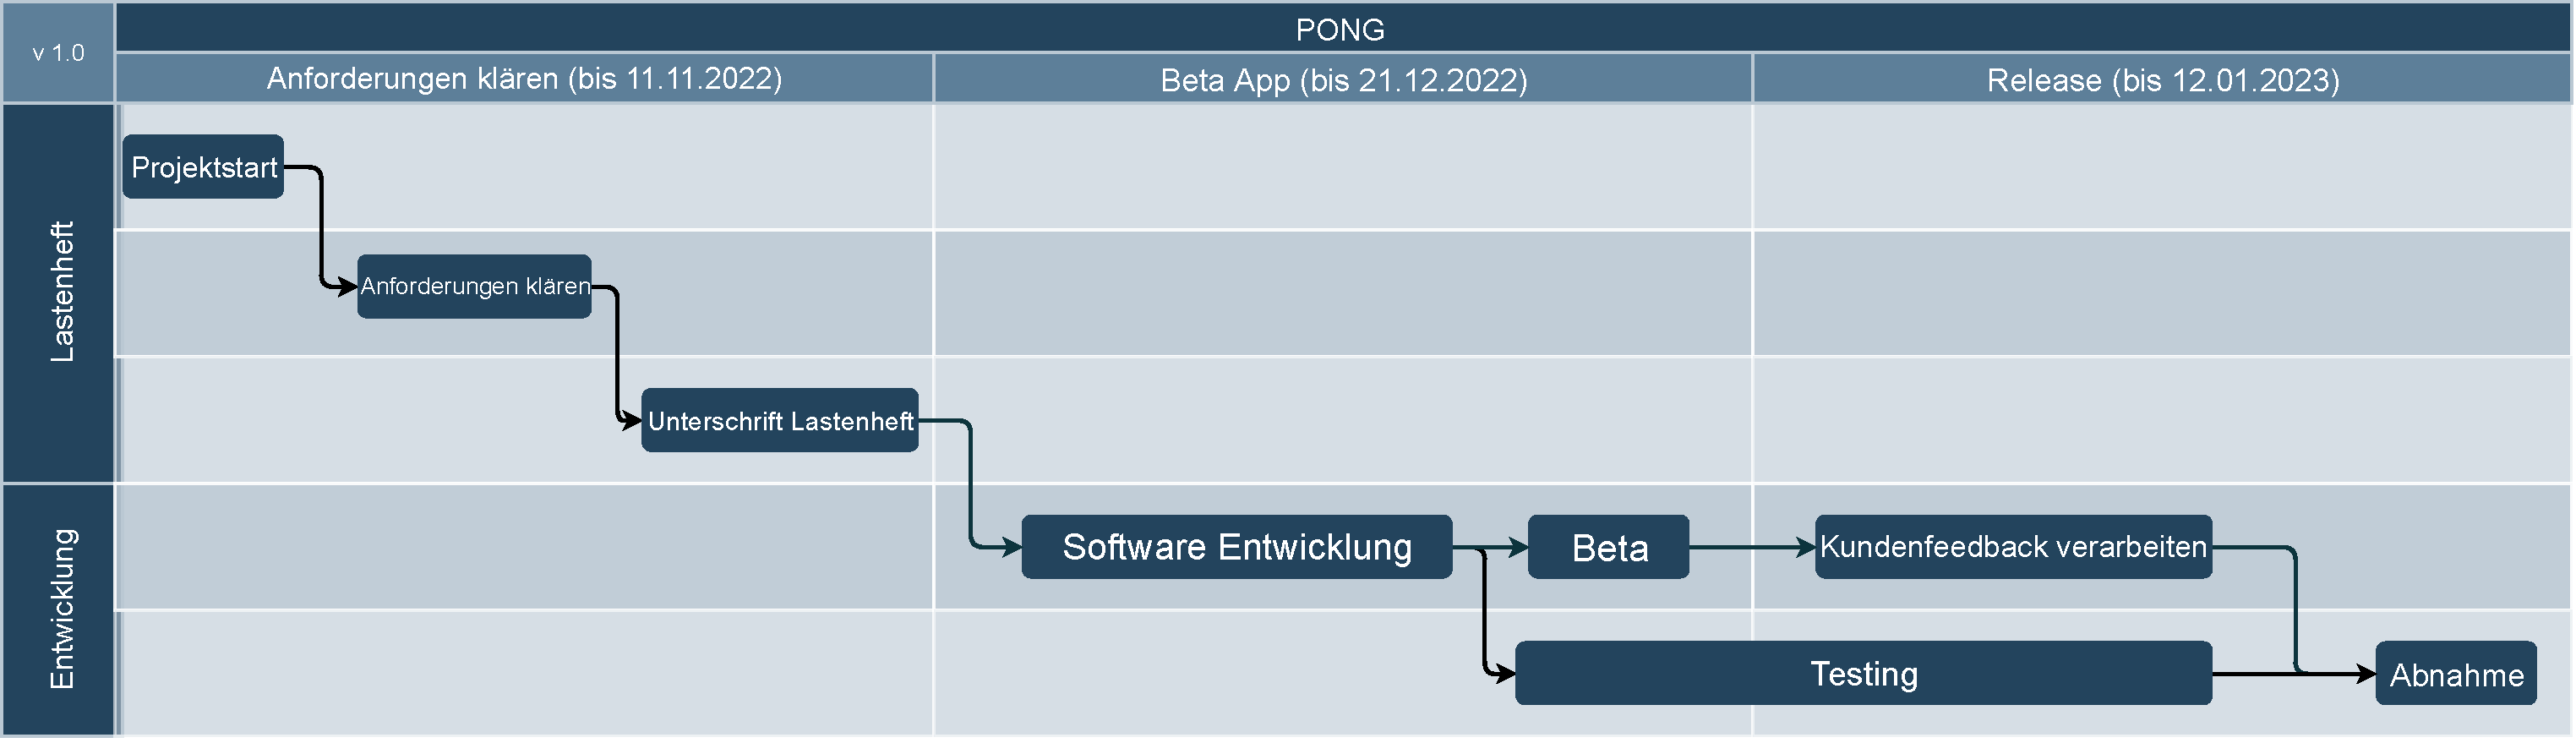
\includegraphics[width=\textwidth]{pdfs/ZeitlicherAblauf.pdf}
    \captionof{figure}{Zeitplan Übersicht}\label{fig:dia:zeitplan}
\end{figure}


    \clearpage

    \section{Zielbestimmung}\label{sec:bestimmung}
        \subsection{Zweck}
            Der \gls{spieler} verwendet das Spiel PONG hauptsächlich als Gelegenheitsspiel, welches z.B. in Pausen die Langeweile vertreibt. 
Des Weiteren kann der \gls{spieler} das Spiel verwenden, um sich mit anderen durch Top-Scores zu messen oder um der Realität zu entfliehen und Spaß zu haben. 
Der gesellschaftliche Effekt des Austauschs von Highscores und bereits freigeschalteten \glspl{skin} ist ebenfalls ein zentraler Punkt. Die stetige Verbesserung der eigenen Leistung und der dadurch entstehende Ehrgeiz ist ein weiterer Faktor, welcher die \gls{spieler} motiviert.
\\
PONG ist kostenlos erhältlich und kann von Menschen aus allen Lebens\-bereichen genossen werden.


        \subsection{Nutzen}
            Das Spiel PONG ermöglicht es dem \gls{spieler} sich im Spiel zu verbessern, mit anderen zu konkurrieren, und bei Gelegenheit der Realität zu entfliehen.
\\
In der App kann der \gls{spieler} \glspl{skin} freischalten, wodurch der Spielspaß erhalten bleibt und der \gls{spieler} eine Langzeitmotivation erhält. Außerdem gibt es eine Monetarisierung durch Werbung.

Durch die kostenfreie Bereitstellung der App erhofft sich \hyperref[sec:auftraggeber]{der Auftraggeber} eine großflächige
Ausbreitung innerhalb der gewählten Zielgruppe. Dabei liegt der langfristige Nutzen hauptsächlich im Ertrag durch Werbeeinnahmen.
Diese fallen an, sofern der \gls{spieler} sich dazu entschließt ein Werbevideo anzuschauen, um nach dem ersten Verlieren aller \gls{leben} weiterspielen zu können (siehe dazu Aktivitätsdiagramm \hyperref[fig:dia:ads]{u12}, Game-Over Menü \hyperref[subsec:u11-gameOverMenu]{u11}).

    \clearpage

    \section{Produkteinsatz}\label{sec:einsatz}
        \subsection{Anwendungsbereich}
        Nach dem Start der App \gls{muss} dem Spieler das Hauptmenü angezeigt werden.
Von dort aus \gls{muss} er die folgenden Optionen haben:
\begin{itemize}
    \item einen Button zum Starten eines neuen Spieldurchlaufs
    \item einen Button zum Anzeigen der \gls{Top10}
    \item einen Button zum Einsehen und Nutzen des Stores
    \item einen Button zum Einsehen der Credits
    \item einen Button zum Einsehen der Achievements\OPT{*}
\end{itemize}

Außerdem wird ein Button zur Sprachauswahl als \gls{niceToHave} betrachtet.\\

Im Folgenden werden die einzelnen Anforderungen weiter erläutert:

Der Spieler \gls{muss} in der Lage sein, den Screen zum Starten eines neuen Spiel\-durchlaufs durch den zugehörigen Button zu erreichen. Auf diesem
Screen \gls{muss} der Spieler den Spielmodus auswählen können. Dem Spieler \gls{muss} es danach möglich sein, die Schwierigkeit auszusuchen.
Nach diesen Schritten kommt der Spieler direkt auf das Spielfeld und der Spieldurchlauf beginnt.

Möchte der Spieler das Spiel pausieren, so ist dies mit einem Pause-Button möglich, welcher oben rechts auf dem Bildschirm platziert sein \gls{muss}.
Verliert der Spieler alle \gls{leben}, so \gls{muss} er einmalig die Möglichkeit haben, optional durch die Anzeige eines Werbevideos ein weiteres Leben zu erhalten und weiterzuspielen.
Ist ein Spieldurchlauf beendet und der erreichte Score ist in den \gls{Top10}, so \gls{muss} der Spieler die Möglichkeit haben, seinen Namen in Verbindung mit dem erreichten Score einzutragen.

Entscheidet sich der Spieler dazu, die derzeitigen \gls{Top10} einzusehen, so \gls{muss} er dazu in der Lage sein, diese durch einen Button im Hauptmenü aufzurufen.

Möchte der Spieler den Store besuchen und/oder neue \glspl{skin} auswählen, \gls{muss} er diesen Bereich ebenfalls von dem Hauptmenü aus erreichen können. 
Im Store \gls{muss} es dem Spieler möglich sein, aus einem von mindestens fünf \glspl{skin} für \gls{ball}, \gls{tail}, \gls{balken} und Spiel-Hintergrund auszuwählen.

Um die Credits der PONG-App einzusehen, \gls{muss} der Spieler vom Hauptmenü aus fähig sein, zu einem Credits-Screen zu gelangen. Dort findet er die Namen der Personen, die an der Entwicklung der App beteiligt waren sowie das Copyright.

Der \gls{spieler} \gls{sollte} in der Lage sein, über einen Button im Hauptmenü seine Achievements einsehenen zu können.

Figure~\ref{fig:use-case-diagram} stellt das UseCase diagramm zur App PONG dar:

\begin{figure}[h!]
    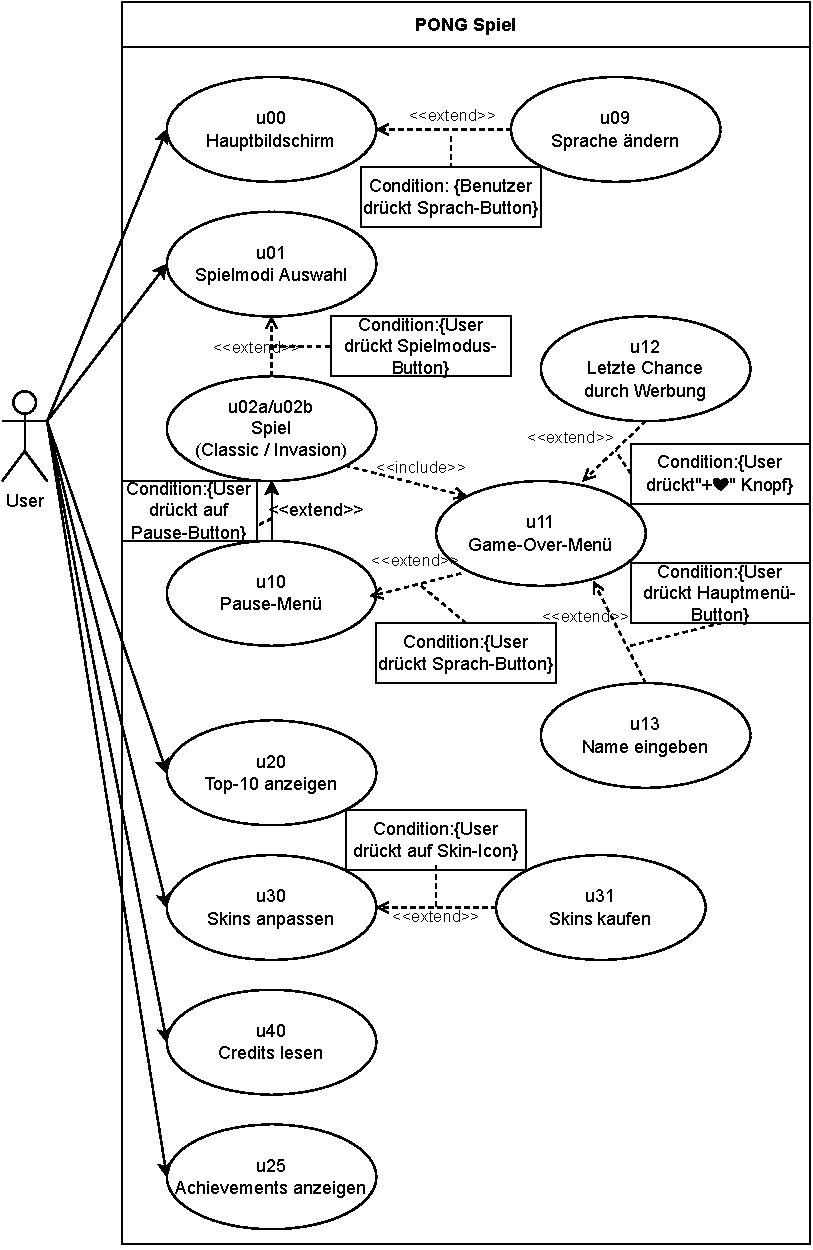
\includegraphics[width=\textwidth]{diagramme/pdf/UML-K4-UseCase.pdf}
    \caption{Use Case Diagramm - PONG}
    \label{fig:use-case-diagram}
\end{figure}

\clearpage
        \subsection{Zielgruppen \& Anwender}
        Es sollen Menschen angesprochen werden, die Interesse an Mobile-Games haben und diese spielen.
Der Spieleklassiker PONG wird neu interpretiert und auf Menschen aus allen Lebensbereichen ausgeweitet.
Junge \gls{spieler} werden durch modernes Design und ältere \gls{spieler} durch das nostalgische Gefühl erreicht.
\\
Die einfache Bedienung ermöglicht es dem \gls{spieler}, schnell und einfach auf das Spiel zuzugreifen 
und somit Wartezeiten und Pausen angenehmer überbrücken zu können.
Angesprochen werden \gls{spieler} aller Altersklassen und jeglichen Geschlechts, die im Besitz eines Smartphones sind.
\\
Um finanzielle Barrieren zu verhindern und die Zielgruppe diesbezüglich nicht einzuschränken, wird die App kostenfrei veröffentlicht.

        \subsection{IST-Zustand des Kunden}
        PONG ist ein Klassiker der Spielindustrie und wurde bereits dutzende Male neu aufgelegt.
Es gibt Desktopanwendungen, Webanwendungen und Mobile Apps. Der Großteil arbeitet aber mit dem Mehrspieler-Prinzip, sodass entweder zwei Spieler gegeneinander oder ein Spieler gegen die KI spielt.

PONG als Klassiker mit moderner Grafik, als Singeplayer-Spiel mit modernem In-Game-Store, verschiedenen Spielmodi und verschiedenen Schwierigkeitsstufen gibt es in der Kombination noch nicht. 
        \clearpage
        \subsection{SOLL-Zustand des Kunden}
        Der letztendliche SOLL-Zustand ergibt sich final aus den \hyperref[sec:requirements]{Requirements} (Kapitel \ref{sec:requirements}).
Im Allgemeinen lässt sich die Applikation wie folgt zusammenfassen:

\begin{itemize}
    \item Die App muss aus einem Startbildschirm, Spiel-, Store-, \gls{Top10} und Credits-Screen bestehen.
    \item Vom Startbildschirm, müssen Spiel, Store, \gls{Top10} und Credits durch Buttons erreichbar sein.
    \item Auf jedem Screen muss es einen Zurück-Button geben.
    \item Das Spiel muss Singleplayer und Hochkant sein.
    \item Es \gls{sollte} aus zwei Spielmodi: \gls{classicMode} und \gls{invasionMode} ausgewählt werden können.
    \item Classic und Invasion sollen aus den klassischen Elementen: Ball und Balken bestehen.
    \item Im Invasion Modus sollen die Kästchen eine bestimmte Anzahl von Malen getroffen werden, um zerstört zu werden.
    \item Pro Spielmodus muss es drei verschiedenen Schwierigkeitsstufen geben: "Easy", "Medium" und "Hard".
    \item Des Weiteren, muss es \glspl{powerup} geben.
    \item Unabhängig von Modus muss das Spiel jederzeit durch einen Button pausierbar sein.
    \item Sobald der Ball unterhalb des Balkens ist, muss der Spieler ein Leben verlieren.
    \item Wenn alle drei Leben aufgebraucht sind, muss es eine einmalige Chance geben, ein weiteres Leben durch das Anschauen einer Werbung zu bekommen.
    \item Falls der Spieler einen neuen Highscore erreicht hat, muss es nach dem Spiel die Möglichkeit geben seinen Namen einzutragen.
    \item Nach jedem Spiel muss dem Spieler sein Score und die verdienten Coins angezeigt werden.
    \item Im Store muss man mit Coins, Skins für Ball, Ball-Schweif, Balken und Hintergrund kaufen und auswählen können.
    \item Der Top-10-Screen muss die Highscores, Namen, Spielmodi und Schwie\-rig\-keits\-stufen anzeigen.
    \item Im Credits-Screen müssen die Namen von Personen, die an der Entwicklung der App gearbeitet haben und das Copyright, angezeigt werden.
\end{itemize}

    \clearpage

    \section{Produktfunktionen}\label{sec:funktionen}
        \subsection{Einleitung}\label{subsec:funktionenEinleitung}
        
In diesem Kapitel ist der genaue Ablauf jeglicher Funktionen des Spiels beschrieben. Die Aktivitäten ‘u‘ stehen für die jeweiligen Screens und Overlays. 
Alle mit ‘a‘ markierten Felder sind Funktionen des Spiels, die vom \gls{spieler} genutzt werden können. Alle mit ‘d‘ markierten Felder sind vom System ausgeführte Funktionen. 
 
\textit{
    Hinweis: Die Beschreibungen in diesem Kapitel (\ref{sec:funktionen}) geben nur die Abläufe der jeweiligen Aktivitäten an und
    sind kein Indikator dafür, ob die genannten Funktionen Pflicht (\gls{muss}) oder optional (\gls{sollte} / \gls{kann}) sind.
    Alle funktionalen Anforderungen können aus der Requirements-Tabelle (Kapitel \ref{sec:requirements}) entnommen werden.  
}

        \subsection{Alle Funktionen, beschrieben aus Anwendersicht}\label{subsec:alleFunktionen}
        

\subsubsection{Aktivität u00 - App-Start / Hauptmenü}
\vspace*{1cm}

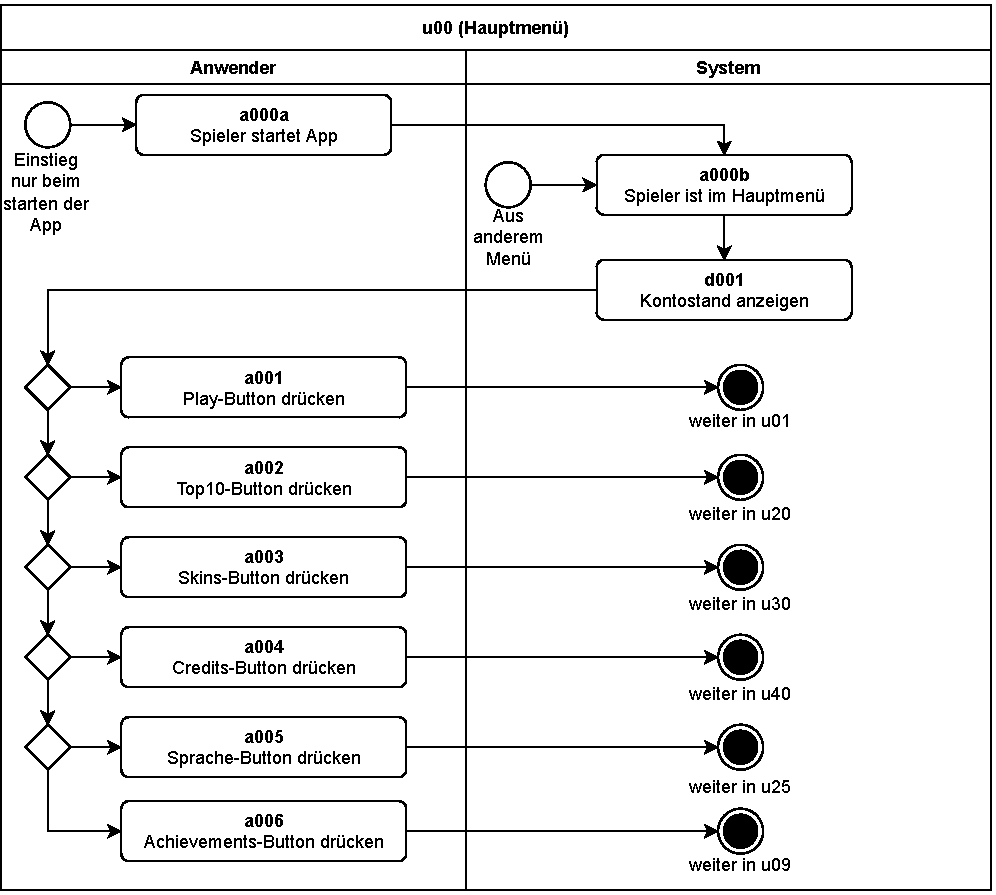
\includegraphics[width=\linewidth]{diagramme/pdf/UML-Activity-u00.pdf}
\captionof{figure}{Aktivität u00 - App-Start / Hauptmenü}\label{fig:dia:mainMenu}
\vspace*{0.5cm}

Figure \ref{fig:dia:mainMenu} stellt den Ablauf der Aktivität u00 dar und in Kapitel \ref{dialog:hauptmenu} wird die dazugehörige Benutzeroberfläche dargestellt. Nach der Installation hat der \gls{spieler} die Möglichkeit, mit einem Klick auf die Anwendung (zu finden in der Liste installierter Apps des Mobilgeräts) das Spiel zu starten. 
Nach maximal fünf Sekunden Ladezeit befindet sich der Spieler dann automatisch im Hauptmenü. Im \hyperref[fig:dia:mainMenu]{Hauptmenü} stehen dem \gls{spieler} fünf verschiedene Buttons zur Verfügung, die ihn zu anderen Screens leiten. Mit dem Play-Button gelangt man zur Spielauswahl. Über den \gls{Top10} Button kann man sich die zehn besten Spiel\-durch\-läufe im \gls{classicMode} und \gls{invasionMode} anschauen.

\vspace{1em}

Im Spiel sind außerdem \glspl{skin} enthalten, die man nach Klicken des Skins-Buttons anschauen und kaufen kann. Mit dem Credits-Button gelangt man zu einem Screen, der ein paar Worte der Entwickler enthält und alle Mitwirkenden am Spiel auflistet. Über den Sprache-Button öffnet sich ein Overlay direkt über dem \hyperref[fig:dia:mainMenu]{Hauptmenü}, dass dem \gls{spieler} die Möglichkeit gibt, die Sprache der gesamten App zu ändern. Die Standard-Sprache ist Englisch. Zuletzt gibt es noch ein weiteres Fenster für Achievements, das über den Achievements-Button aufgerufen werden kann.


\clearpage

\subsubsection{Aktivität u01 - Spielmodus Einstellungen}

\vspace*{1cm}
   
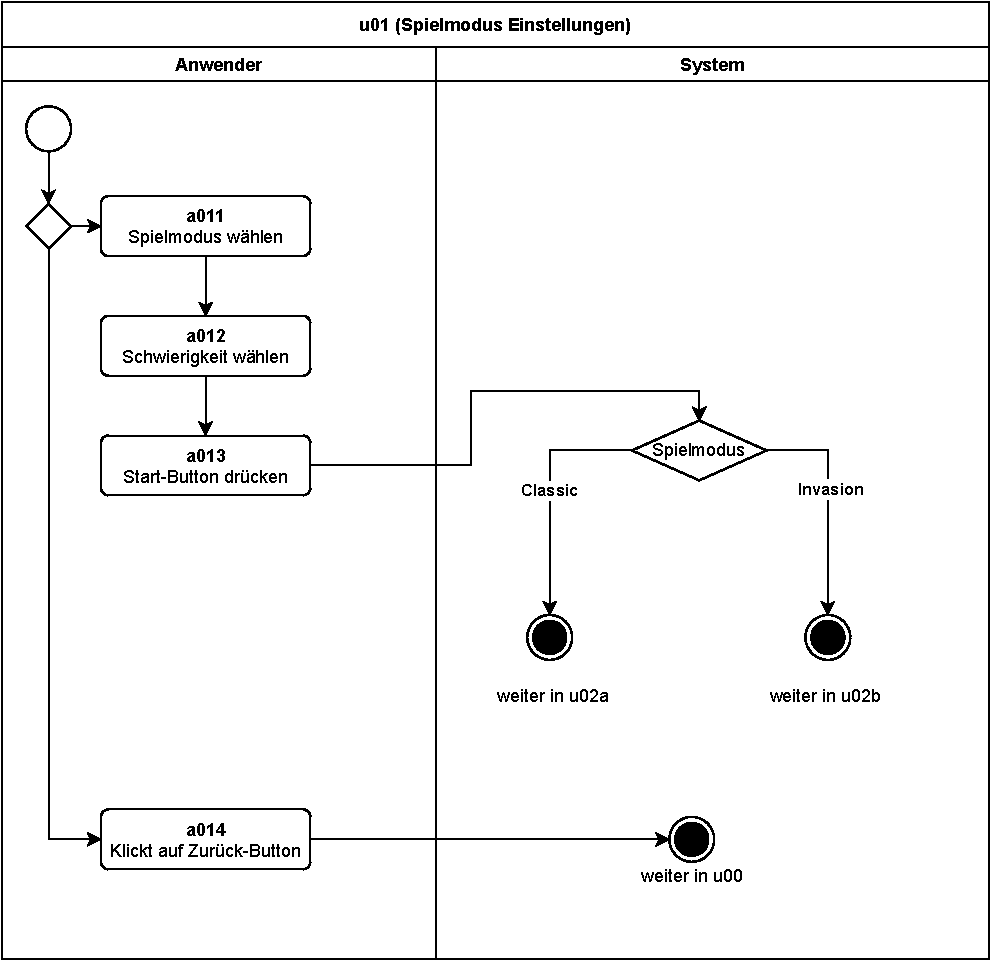
\includegraphics[width=\linewidth]{diagramme/pdf/UML-Activity-u01.pdf}
\captionof{figure}{Aktivität u01 - Spielmodus Einstellungen}\label{fig:dia:gameMode}
\vspace*{0.5cm}

Figure \ref{fig:dia:gameMode} stellt den Ablauf der Aktivität u01 dar und in Kapitel \ref{dialog:einstellungen} wird die dazugehörige Benutzeroberfläche dargestellt.
Hat der \gls{spieler} den Play-Button gedrückt, so gelangt er in ein neues Fenster, dass ihm die Möglichkeit bietet, den Spielmodus (\gls{classicMode}/\gls{invasionMode}) und die Schwierigkeit (Easy, Medium, Hard) einzustellen. Drückt der \gls{spieler} dann den Start-Button, wird eine neue Spielrunde mit den ausgewählten Einstellungen geladen. Über den Zurück-Button gelangt man wieder in das \hyperref[fig:dia:mainMenu]{Hauptmenü} und die Einstellungen werden verworfen.

\clearpage

\subsubsection{Aktivität u02a - Spiel Classic}

\vspace*{1cm}

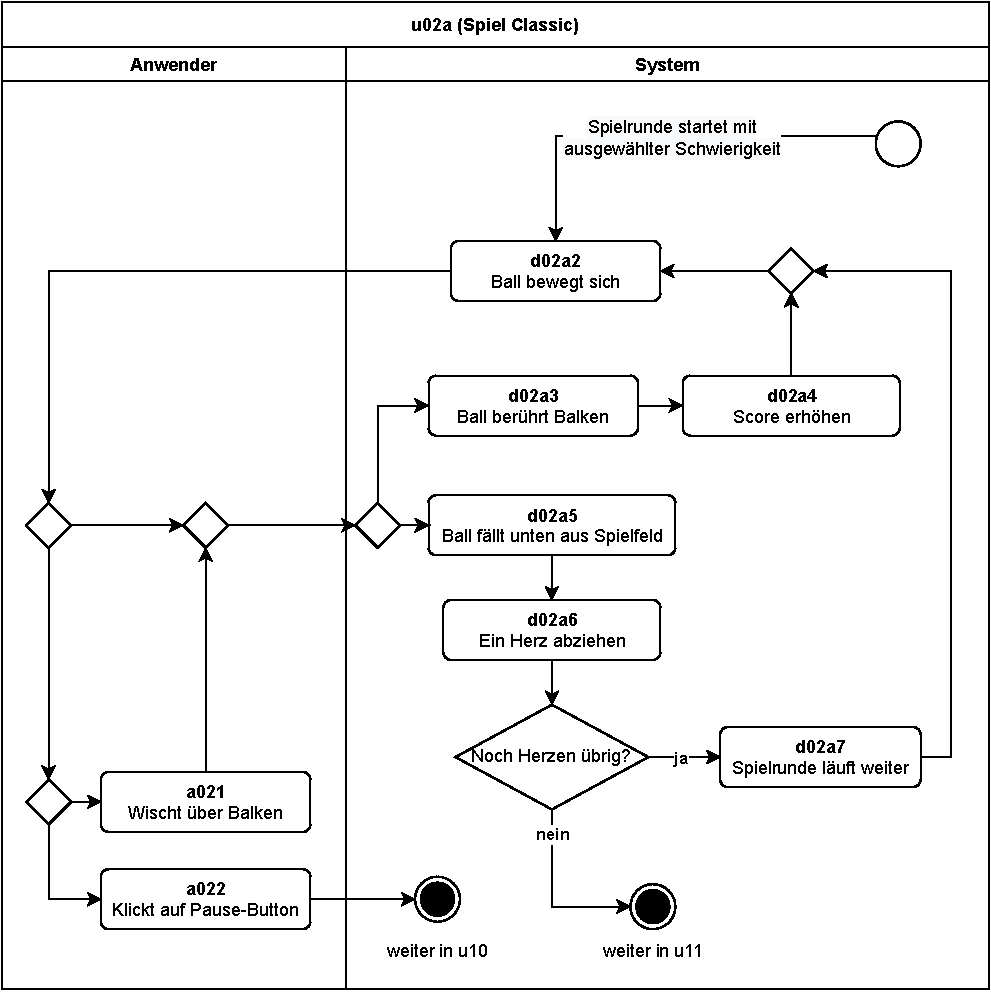
\includegraphics[width=\linewidth]{diagramme/pdf/UML-Activity-u02a.pdf}
\captionof{figure}{Aktivität u02a - Spiel Classic}\label{fig:dia:classic}
\vspace*{0.5cm}

Figure \ref{fig:dia:classic} stellt den Ablauf der Aktivität u02a dar und in Kapitel \ref{dialog:classic} wird die dazugehörige Benutzeroberfläche dargestellt.
Im \gls{classicMode} muss der \gls{spieler} den \gls{ball} mithilfe des \glspl{balken} im \gls{spielfeld} halten, indem er diesen durch Wischen auf dem Screen nach links und rechts bewegt. Beim Starten einer neuen Spielrunde wird diese mit den ausgewählten Einstellungen (Easy/Medium/Hard) initialisiert und der Ball spawnt. Berührt der \gls{ball} den \gls{balken}, die Wände oder Decke des Spielfelds, so prallt er ab und ändert seine Richtung abhängig vom Auftreffwinkel und Auftreffpunkt. Außerdem wird der Score jedes Mal erhöht, wenn der \gls{ball} den \gls{balken} trifft.
Fällt der Ball unten aus dem \gls{spielfeld}, so verliert der Spieler ein Leben (Startet mit 3), der \gls{ball} wird wieder in die Mitte gesetzt und die Runde läuft weiter. Sollte der \gls{spieler} jedoch drei Leben verlieren, so ist die Runde vorläufig zu Ende und der Game-Over Screen wird aufgerufen.
Der Spieler hat jedoch während der gesamten Zeit immer die Möglichkeit zu pausieren und gegebenenfalls die Runde frühzeitig zu beenden.  


\clearpage
\subsubsection{Aktivität u02b - Spiel Invasion}

\vspace*{1cm}

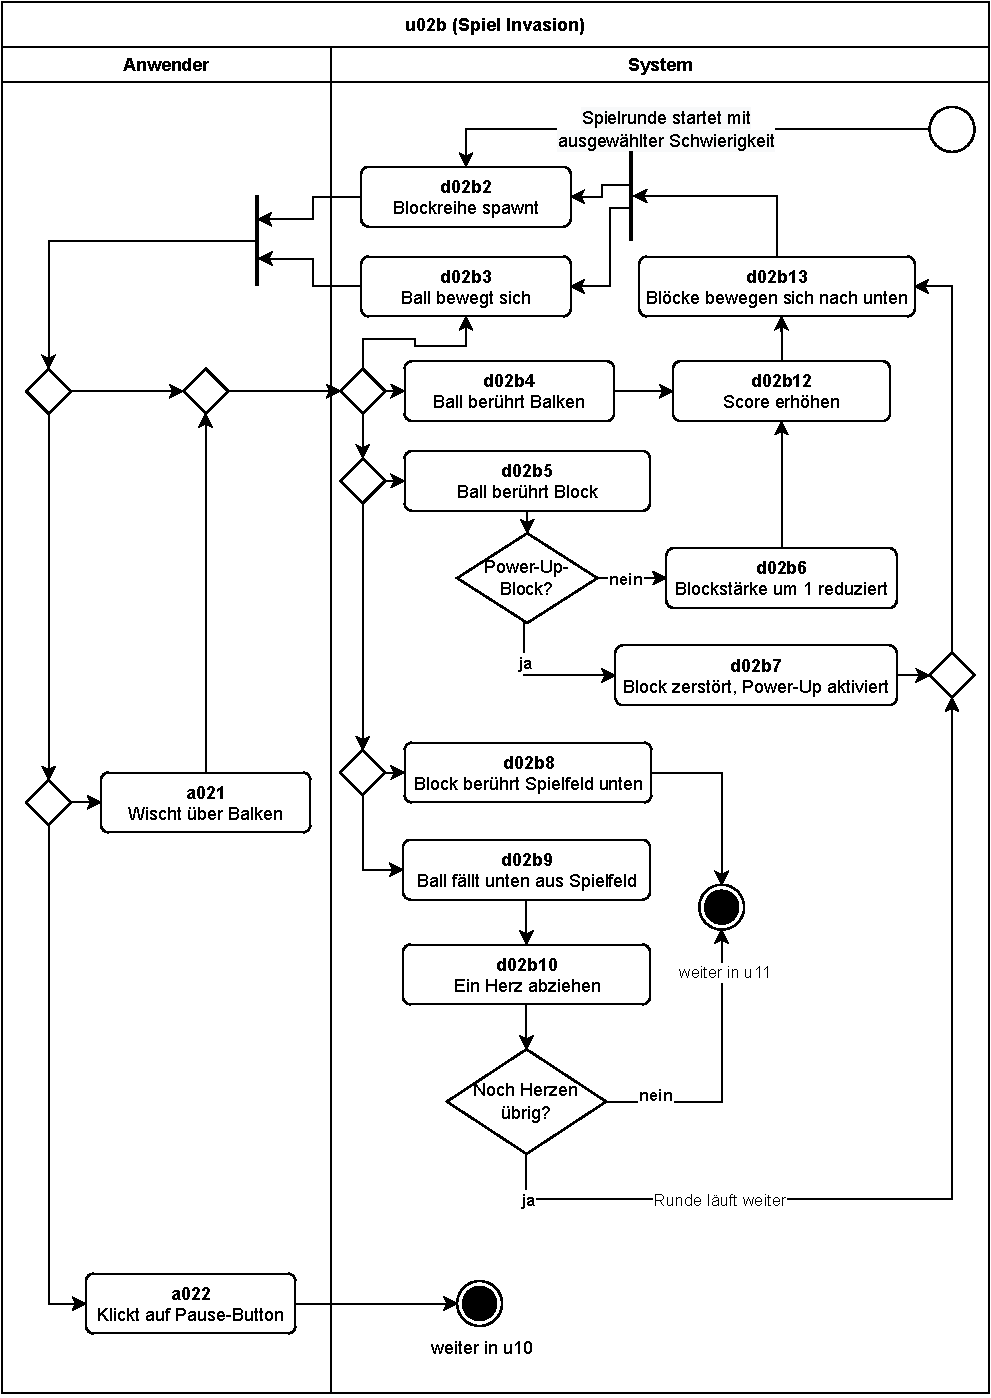
\includegraphics[width=\linewidth]{diagramme/pdf/UML-Activity-u02b.pdf}
\captionof{figure}{Aktivität u02b - Spiel Invasion}\label{fig:dia:invasion}
\vspace*{0.5cm}


\textit{Der Spielmodus Invasion und der damit verbundene Screen sind optional.}
\\
Figure \ref{fig:dia:invasion} stellt den Ablauf der Aktivität u02b dar und in Kapitel \ref{dialog:invasion} wird die dazugehörige Benutzeroberfläche dargestellt.
Der \gls{invasionMode} ist eine Erweiterung zum \gls{classicMode}. Ab Rundenstart spawnt periodisch eine Reihe an Blöcken verschiedener Stärke und vereinzelt mit Power-Ups für den \gls{spieler}. Diese Blöcke müssen mehrmals, je nach der Stärke des Blocks, vom \gls{ball} getroffen werden, um sie zu zerstören. Zerstört der Spieler einen \gls{powerup}-\gls{block}, so erhält der \gls{ball} oder der \gls{spieler} für kurze Zeit eine besondere Eigenschaft (siehe 9.2.1). 
Zusätzlich muss der Spieler darauf achten, dass kein Block den unteren Spielfeldrand berührt. Ansonsten verliert er alle seine Leben und wird direkt zum Game-Over-Menü geleitet. Alle anderen Spielabläufe des \gls{invasionMode} sind identisch zu dem des \gls{classicMode} (5.1.3).


\clearpage

\subsubsection{Aktivität u09 - Sprachauswahl}

\vspace*{1cm}

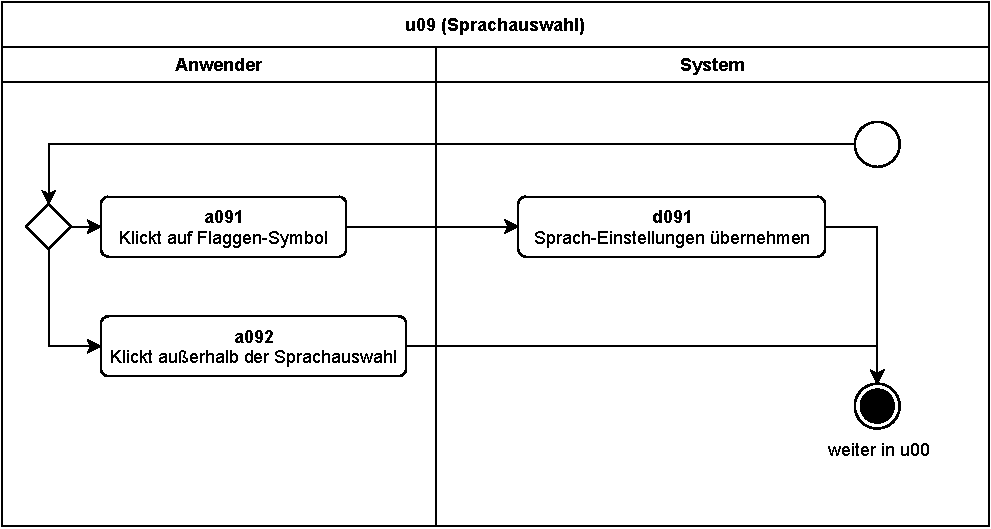
\includegraphics[width=\linewidth]{diagramme/pdf/UML-Activity-u09.pdf}
\captionof{figure}{Aktivität u09 - Sprachauswahl}\label{fig:dia:language}
\vspace*{0.5cm}

\textit{Die Sprachauswahl und das damit verbundene Overlay sind optional.}
\\
Figure \ref{fig:dia:language} stellt den Ablauf der Aktivität u09 dar und in Kapitel \ref{dialog:Sprachauswahl} wird die dazugehörige Benutzeroberfläche dargestellt.
Wurde der Sprache-Button im Hauptmenü gedrückt, öffnet sich ein Overlay. Darin hat der \gls{spieler} die Möglichkeit, die Sprache des Spiels zu ändern, indem er auf eine der verfügbaren Flaggen klickt. Die Standardeinstellung der Sprache ist Englisch. Durch das Klicken außerhalb der Sprachauswahl kommt der \gls{spieler} wieder in das \hyperref[fig:dia:mainMenu]{Hauptmenü} zurück.

\clearpage


\subsubsection{Aktivität u10 - Pause-Menü}


\vspace*{1cm}

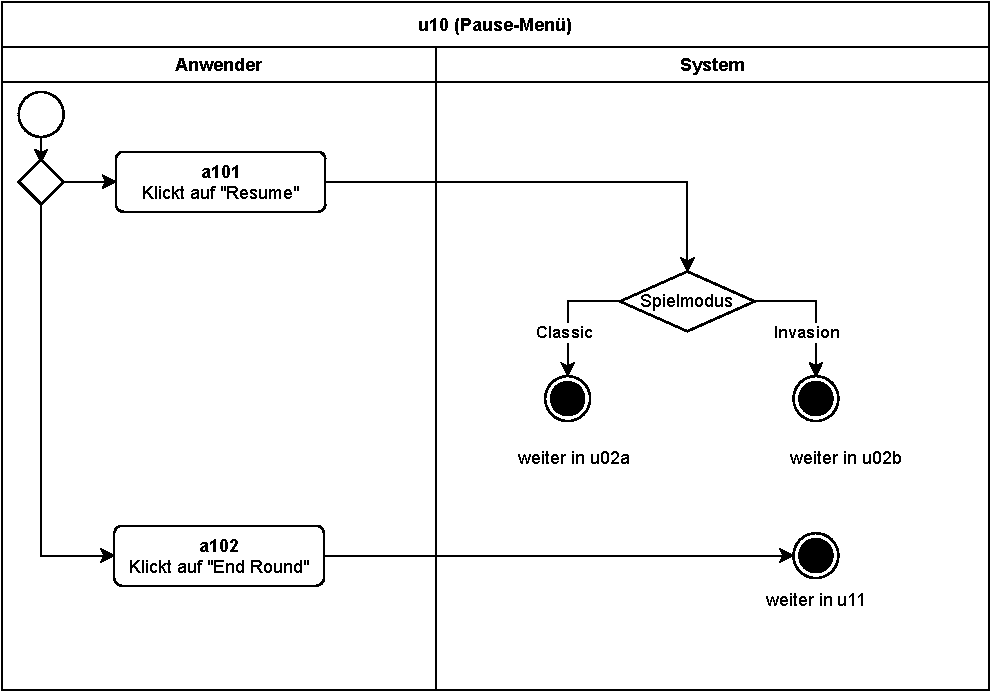
\includegraphics[width=\linewidth]{diagramme/pdf/UML-Activity-u10.pdf}
\captionof{figure}{Aktivität u10 - Pause-Menü}\label{fig:dia:pause}
\vspace*{0.5cm}

Figure \ref{fig:dia:pause} stellt den Ablauf der Aktivität u10 dar und in Kapitel \ref{dialog:pause} wird die dazugehörige Benutzeroberfläche dargestellt.
Während einer aktiven Spielrunde hat der \gls{spieler} die Möglichkeit zu pausieren. Dann wird das Spiel angehalten und ein Overlay öffnet sich. Darin kann der Spieler entweder den Resume-Button klicken, um die jeweilige Runde fortzusetzen, oder auf "End-Round" klicken, um die Runde frühzeitig zu beenden.

\clearpage

\subsubsection{Aktivität u11 - Game-Over-Menü}\label{subsec:u11-gameOver}

\vspace*{1cm}

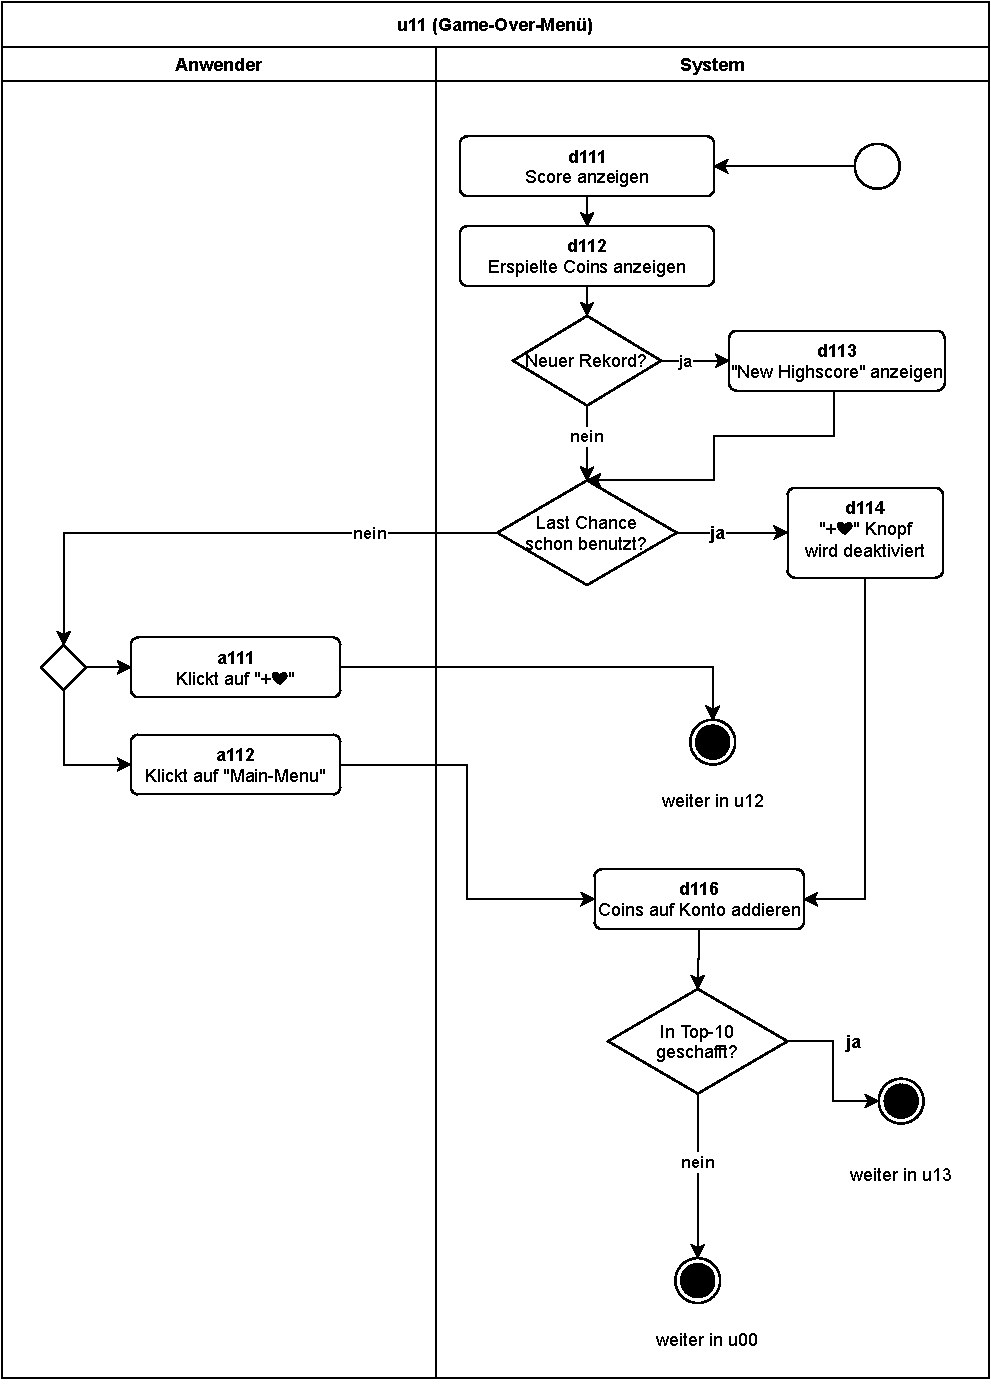
\includegraphics[width=\linewidth]{diagramme/pdf/UML-Activity-u11.pdf}
\captionof{figure}{Aktivität u11 - Game-Over-Menü}\label{fig:dia:gameOver}
\vspace*{0.5cm}

Figure \ref{fig:dia:gameOver} stellt den Ablauf der Aktivität u11 dar und in Kapitel \ref{subsec:u11-gameOverMenu} wird die dazugehörige Benutzeroberfläche dargestellt.
Hat der \gls{spieler} alle seine Leben verloren, oder die Runde im Pause-Menü frühzeitig beendet, so kommt er automatisch in das Game-Over-Menü. Hier werden die erspielten Coins und der bisher erreichte Score angezeigt. Hat er in der Runde einen höheren Score erreicht als einer der Scores in der \gls{Top10} Liste, bekommt der \gls{spieler} die Nachricht „New Highscore“ auf dem Screen angezeigt.

\vspace{1em}

Hat der \gls{spieler} noch keine „Last Chance“ genutzt, so bietet ihm das System einmalig die Möglichkeit, einen Werbeclip zu schauen, um nochmal ein Leben zu erhalten und die Runde fortzusetzen. Verliert der \gls{spieler} auch dieses Leben ist die Runde endgültig zu Ende. Danach werden die erspielten Coins automatisch auf das Spiel-Konto addiert und das System prüft, ob der Score des Spielers hoch genug ist, um in die \gls{Top10} zu kommen. Ist dies der Fall, so wird eine Namenseingabe angezeigt, in der der \gls{spieler} seinen Namen eingeben kann. Hat der \gls{spieler} keine \gls{Top10} Platzierung erreicht, wird das \hyperref[fig:dia:mainMenu]{Hauptmenü} geöffnet.
\clearpage

\subsubsection{Aktivität u12 - Werbung}\label{subsec:u12-ads}

\vspace*{1cm}

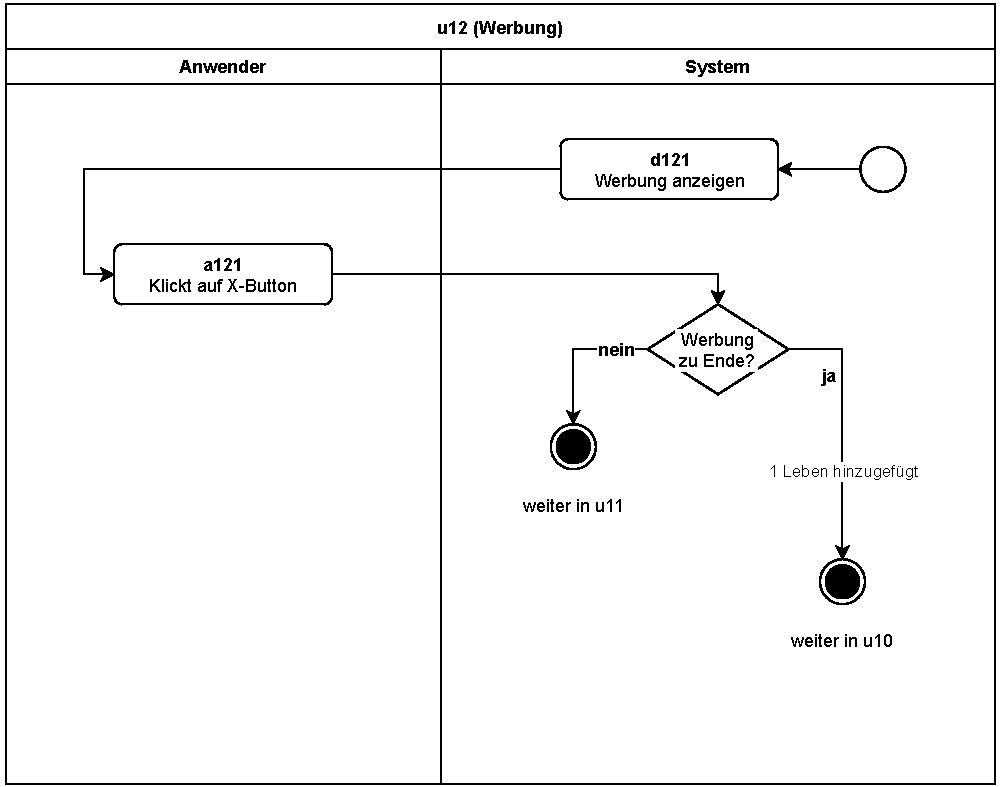
\includegraphics[width=\linewidth]{diagramme/pdf/UML-Activity-u12.pdf}
\captionof{figure}{Aktivität u12 - Werbung}\label{fig:dia:ads}
\vspace*{0.5cm}

Figure \ref{fig:dia:ads} stellt den Ablauf der Aktivität u12 dar und in Kapitel \ref{dialog:Werbung} wird die dazugehörige Benutzeroberfläche dargestellt.
Entscheidet sich der \gls{spieler} Werbung anzuschauen, so hat er die Möglichkeit, diese über den X-Button wieder zu schließen. Ist die Werbung zu diesem Zeitpunkt noch nicht vollständig durchgelaufen, so wird der \gls{spieler} wieder in das Game-Over-Menü weitergeleitet. Hat er sich die Werbung jedoch vollständig angeschaut, so erhält er ein extra Leben und wird zum Pause-Menü weitergeleitet, sodass die Runde fortgesetzt werden kann. Bei Game-Over durch die Berührung eines Blocks mit dem unteren Spielfeldrand, wird die Spielrunde nach dem schauen der Werbung neu initialisiert.

\clearpage

\subsubsection{Aktivität u13 - Namenseingabe}

\vspace*{1cm}

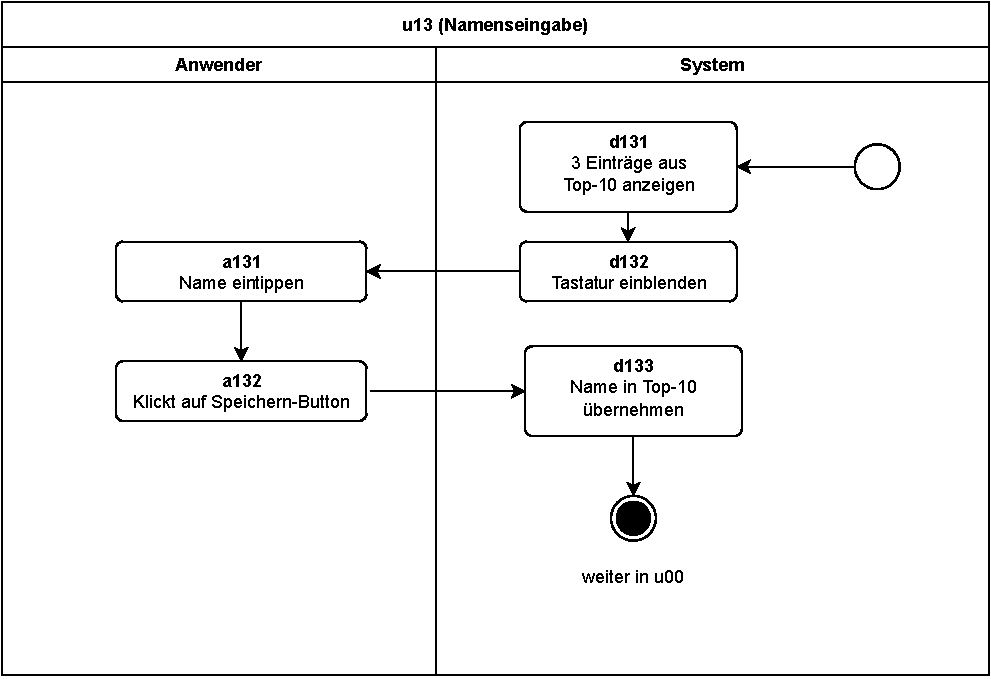
\includegraphics[width=\linewidth]{diagramme/pdf/UML-Activity-u13.pdf}
\captionof{figure}{Aktivität u13 - Namenseingabe}\label{fig:dia:highscore}
\vspace*{0.5cm}

Figure \ref{fig:dia:highscore} stellt den Ablauf der Aktivität u13 dar und in Kapitel \ref{dialog:Namenseingabe} wird die dazugehörige Benutzeroberfläche dargestellt.
Hat der \gls{spieler} nach der Runde eine \gls{Top10} Platzierung erreicht, so wird die Namenseingabe angeboten. Es wird, sofern vorhanden, ein Eintrag der Platzierungen genau vor und einer genau hinter dem des erreichten Scores angezeigt. Unterhalb dieser Anzeige wird die Tastatur
eingeblendet und der \gls{spieler} hat so die Möglichkeit seinen Namen einzutippen und anschließend durch den Klick auf den Speichern-Button seinen Namen in Zusammenhang mit dem Schwierigkeitsgrad und erreichten Score in den \gls{Top10} zu sichern. Danach wird der \gls{spieler} wieder in das \hyperref[fig:dia:mainMenu]{Hauptmenü} geleitet.

\clearpage

\subsubsection{Aktivität u20 - Top-10 Liste}

\vspace*{1cm}

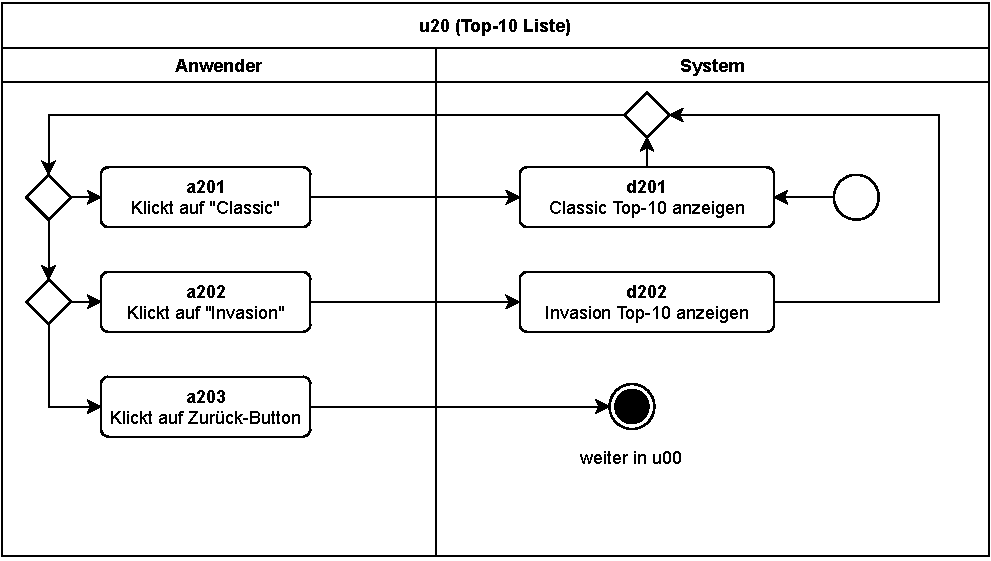
\includegraphics[width=\linewidth]{diagramme/pdf/UML-Activity-u20.pdf}
\captionof{figure}{Aktivität u20 - Top-10 Liste}\label{fig:dia:top10}
\vspace*{0.5cm}

Figure \ref{fig:dia:top10} stellt den Ablauf der Aktivität u20 dar und in Kapitel \ref{dialog:top10} wird die dazugehörige Benutzeroberfläche dargestellt.
Klickt der \gls{spieler} im \hyperref[fig:dia:mainMenu]{Hauptmenü} auf den \gls{Top10}-Button, so werden ihm standardmäßig die 10 höchsten Scores im \gls{classicMode} in Listenform angezeigt. Durch einen Klick auf den Invasion-Button ändert sich die Liste und zeigt dann die 10 höchsten Scores im \gls{invasionMode} an. Analog dazu führt der Classic-Button zur Top-10 Liste des \gls{classicMode} zurück.
Über den Zurück-Button gelangt der \gls{spieler} wieder in das \hyperref[fig:dia:mainMenu]{Hauptmenü}.

\clearpage

\subsubsection{Aktivität u25 - Achievements}

\vspace*{1cm}

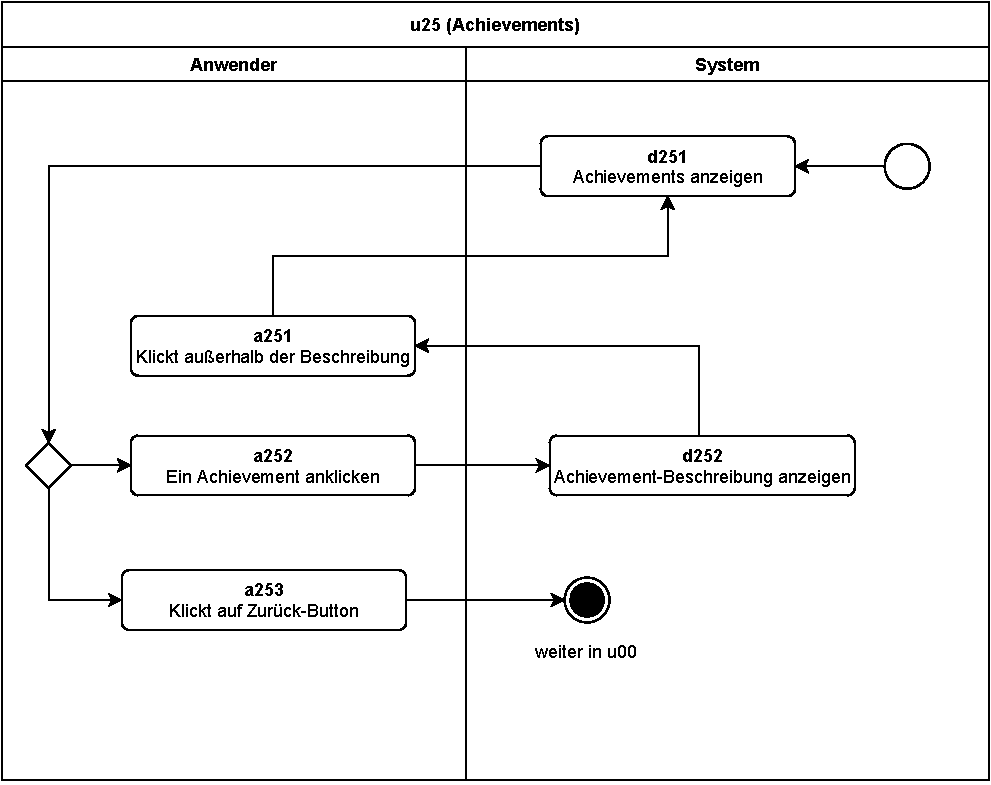
\includegraphics[width=\linewidth]{diagramme/pdf/UML-Activity-u25.pdf}
\captionof{figure}{Aktivität u25 - Achievements}\label{fig:dia:achievements}
\vspace*{0.5cm}

\textit{Die Achievements und der damit verbundene Screen sind optional.}
\\
Figure \ref{fig:dia:achievements} stellt den Ablauf der Aktivität u25 dar und in Kapitel \ref{dialog:Achievements} wird die dazugehörige Benutzeroberfläche dargestellt.
Über den Achievements-Button gelangt der \gls{spieler} auf einen Screen, der alle seine bisher erreichten Achievements anzeigt. Noch nicht erreichte Achievements sind ausgegraut. Wird auf eines der Symbole geklickt, so öffnet sich ein Overlay und der Spieler kann die Beschreibung des jeweiligen Achievements nachlesen. Klickt der Spieler außerhalb des Overlays, kommt er zurück auf die Ansicht aller Achievements. Durch das Klicken des Zurück-Buttons gelangt der Spieler dann wieder in das \hyperref[fig:dia:mainMenu]{Hauptmenü}. 

\clearpage

\subsubsection{Aktivität u30 - Skin-Auswahl}

\vspace*{1cm}

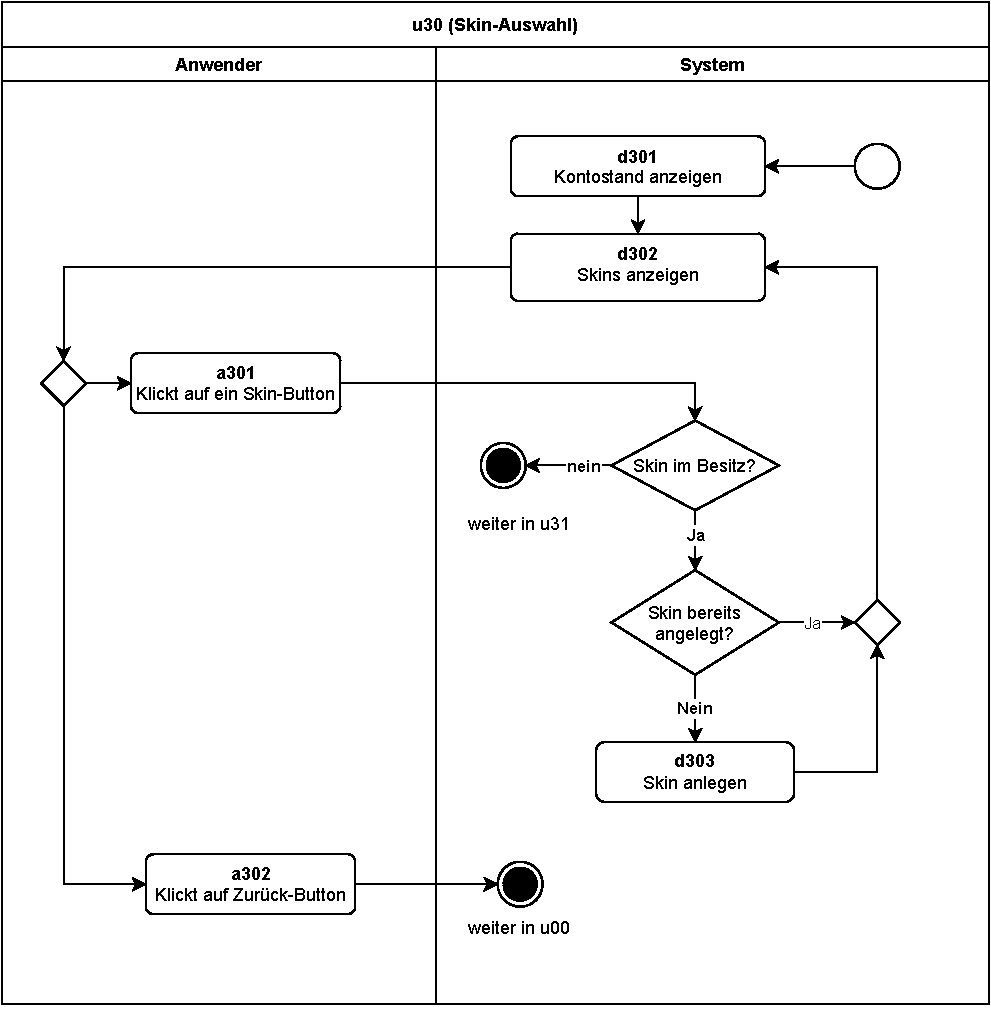
\includegraphics[width=\linewidth]{diagramme/pdf/UML-Activity-u30.pdf}
\captionof{figure}{Aktivität u30 - Skin-Auswahl}\label{fig:dia:skins}
\vspace*{0.5cm}

Figure \ref{fig:dia:skins} stellt den Ablauf der Aktivität u30 dar und in Kapitel \ref{dialog:skins} wird die dazugehörige Benutzeroberfläche dargestellt.
Klickt der Spieler auf den Skins-Button, so gelangt er auf einen Screen, der ihm alle im Spiel verfügbaren \glspl{skin} des \glspl{ball}, des \glspl{tail}, des Balkens und des Hintergrunds anzeigt. Zusätzlich sieht er hier auch seinen aktuellen Kontostand. Durch Klicken eines Skin-Buttons wird ein Overlay geöffnet, das dem \gls{spieler} die Möglichkeit bietet, den \gls{skin} zu kaufen oder anzulegen. Ist der ausgewählte \gls{skin} bereits angelegt, so wird das Overlay nicht geöffnet und der Spieler bleibt auf der Anzeige aller \glspl{skin}.
\clearpage

\subsubsection{Aktivität u31 - Skin-Kauf}

\vspace*{1cm}

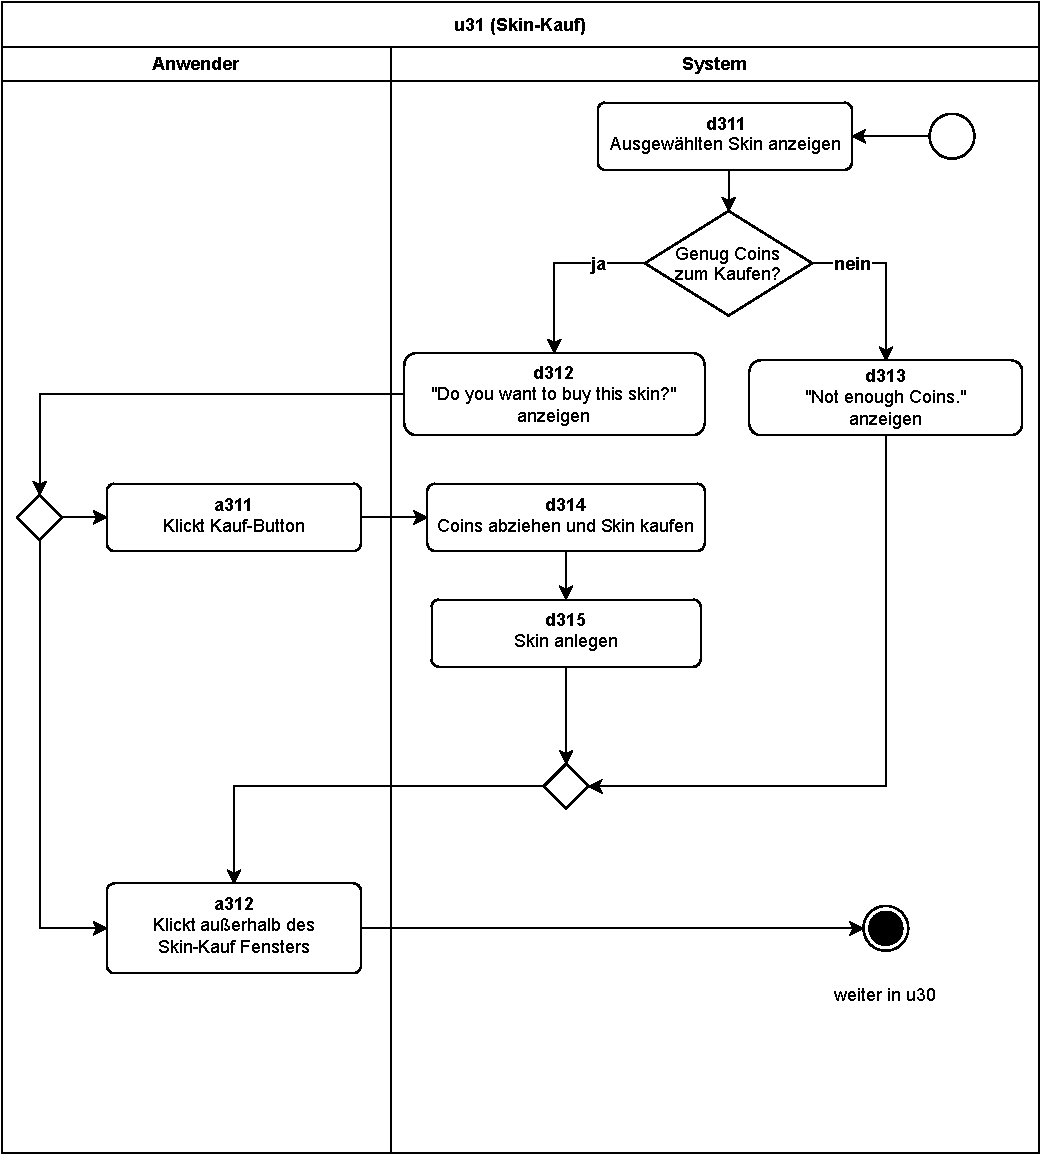
\includegraphics[width=\linewidth]{diagramme/pdf/UML-Activity-u31.pdf}
\captionof{figure}{Aktivität u31 - Skin-Kauf}\label{fig:dia:skinPurchase}
\vspace*{0.5cm}

Figure \ref{fig:dia:skinPurchase} stellt den Ablauf der Aktivität u31 dar und in Kapitel \ref{dialog:skinkauf} wird die dazugehörige Benutzeroberfläche dargestellt.
Hat der \gls{spieler} einen \gls{skin} ausgewählt, so wird ein Overlay geöffnet. Ist der \gls{skin} noch nicht in seinem Besitz, so wird vom System geprüft, ob genügend Coins für den Kauf des \glspl{skin} vorhanden sind. Ist dies der Fall, so wird die Nachricht „Do you want to buy this skin?“ angezeigt. Entscheidet sich dann der \gls{spieler} diesen zu kaufen, so werden die benötigten Coins von seinem Konto abgezogen, der \gls{skin} freigeschaltet und direkt angelegt. 
Fehlen dem \gls{spieler} noch Coins für den \gls{skin}, so zeigt das System die Nachricht „Not enough Coins“ an. Mit einem Klick außerhalb des Overlays kommt der \gls{spieler} dann wieder zurück auf die Anzeige aller \glspl{skin}.

\clearpage

\subsubsection{Aktivität u40 - Credits}

\vspace*{1cm}

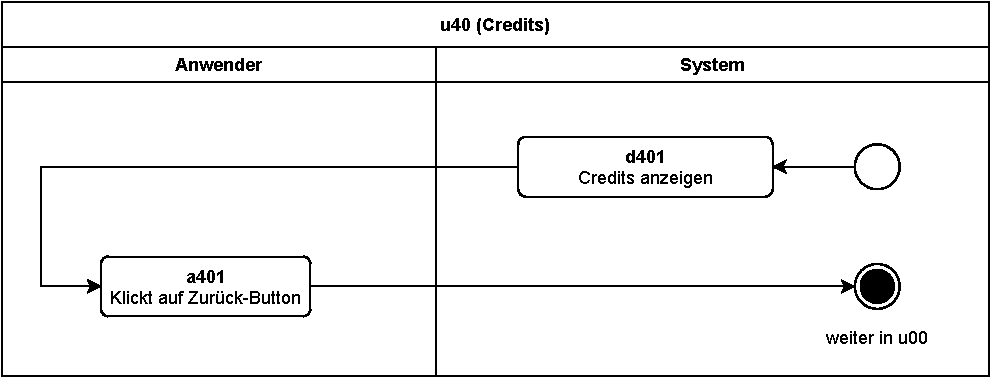
\includegraphics[width=\linewidth]{diagramme/pdf/UML-Activity-u40.pdf}
\captionof{figure}{Aktivität u40 - Credits}\label{fig:dia:credits}
\vspace*{0.5cm}

Figure \ref{fig:dia:credits} stellt den Ablauf der Aktivität u40 dar und in Kapitel \ref{dialog:credits} wird die dazugehörige Benutzeroberfläche dargestellt.
Bei einem Klick auf den Credits-Button muss das System dem \gls{spieler} die Credits anzeigen. 
Dieser enthält paar Worte der Entwickler und listet alle Mitwirkenden am Spiel auf. 
Der \gls{spieler} hat die Möglichkeit, den Credits-Screen durch einen Klick auf den Zurück-Button zu verlassen und das \hyperref[fig:dia:mainMenu]{Hauptmenü} zu erreichen.

\clearpage

        \subsection{Eingabe/Ausgabe}\label{subsec:EinAusgabe}
        Im Folgenden werden Mockups präsentiert, welche das Design und die Benutzer\-ober\-fläche der PONG App darstellen. Kleinere Änderungen an Design und der Benutzer\-ober\-fläche während des Entwicklungsprozesses sind möglich.

\subsubsection{Figure 17 - Icon Legende}
Figure \ref{fig:dia:icons} listet die in der App verwendeten Icons auf.
\vspace*{0.5cm}

\begin{figure}[h!]
    \begin{center}
        \begin{tabular}{ll}
            
\includegraphics[width=1.5em,height=1.5em]{diagramme/assets/Media-Play-256.png} & Start / Fortsetzen \\
            
\includegraphics[width=1.5em,height=1.5em]{diagramme/assets/Media-Pause-256.png} & Pause \\
            
\includegraphics[width=1.5em,height=1.5em]{diagramme/assets/Close-256.png} & Beenden\\
            
\includegraphics[width=1.5em,height=1.5em]{diagramme/assets/Arrow-Left-05-256.png} & Zurück \\
            
\includegraphics[width=1.5em,height=1.5em]{diagramme/assets/Floppy-256.png} & Speichern und Fortfahren \\
            
\includegraphics[width=1.5em,height=1.5em]{diagramme/assets/Money-Coin-02-WF-256.png} & Coins / Kontostand \\
            
\includegraphics[width=1.5em,height=1.5em]{diagramme/assets/Heart-256.png} & Symbolisiert ein Leben \\
            
\includegraphics[width=1.5em,height=1.5em]{diagramme/assets/Globe-256.png} & Sprachauswahl \\
            
\includegraphics[width=1.5em,height=1.5em]{diagramme/assets/Shirt-256.png} & Allgemeines Symbol für Skins \\
            
\includegraphics[width=1.5em,height=1.5em]{diagramme/assets/list.png} & Top-10 Liste \\
            
\includegraphics[width=1.5em,height=1.5em]{diagramme/assets/Trophy-256.png} & Achievements \\
            
\includegraphics[width=1.5em,height=1.5em]{diagramme/assets/Bomb-256.png} & Beispiel für \gls{powerup}-Block \\    
            
\includegraphics[width=1.5em,height=1.5em]{diagramme/assets/Lock-256.png} & Item gesperrt / nicht im Besitz
        \end{tabular}
    \end{center}
    \captionof{figure}{Icon Legende}\label{fig:dia:icons}
\end{figure}
\setlength{\extrarowheight}{0.5em}

\clearpage

\subsubsection{Dialog u00 - Hauptmenü}\label{dialog:hauptmenu}

\begin{figure}[h!]
    \begin{center}
    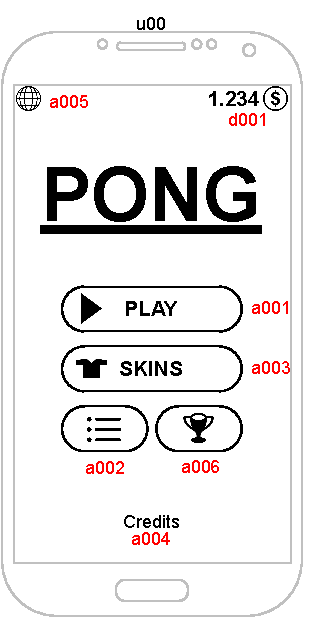
\includegraphics[scale=1.4]{diagramme/pdf/Mockup-u00.pdf}
    \end{center}
    \captionof{figure}{Dialog u00 - Hauptmenü}\label{fig:dia:u00}
\end{figure}

Das Hauptmenü dient dem \gls{spieler} als Ausgangspunkt. Von hier aus kann es möglich sein, die Sprache zu ändern (a005) und die persönlichen Achievements einzusehen (a006). 
Außerdem muss der \gls{spieler} die Anzahl seiner \glspl{coin} ablesen können (d001). Der Play-Button muss den \gls{spieler} zu den Spielmodus Einstellungen führen (a001).
Um die Skin-Auswahl zu öffnen (a003), muss der \gls{spieler} den Skins-Button drücken. Die Top-10 Liste muss sich über den Top-10-Button öffnen lassen (a002). Informationen über das Entwicklerteam muss der \gls{spieler} 
über den Credits-Button abrufen können (a004).
(siehe Fig. \ref{fig:dia:u00})

\clearpage

\subsubsection{Dialog u01 - Spielmodus Einstellungen}\label{dialog:einstellungen}

\begin{figure}[h!]
    \begin{center}
    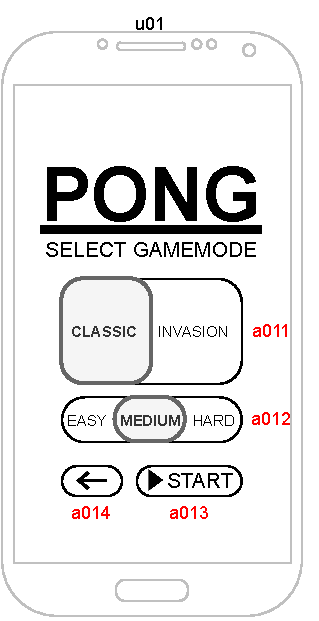
\includegraphics[scale=1.4]{diagramme/pdf/Mockup-u01.pdf}
    \end{center}
    \caption{Dialog u01 - Spielmodus Einstellungen}\label{fig:dia:u01}
\end{figure}

Möchte der \gls{spieler} ein Spiel starten, so muss es zunächst eine Auswahl zwischen den Spielmodi \gls{classicMode} und \gls{invasionMode} geben (a012). Nach der Wahl des Spielmodus muss der \gls{spieler} einen der drei Schwierigkeitsstufen (a011) wählen können.
Zurück zum Hauptmenü muss der \gls{spieler} mit dem Zurück-Button gelangen. Wenn der \gls{spieler} seine Entscheidungen über Spielmodus und Schwierigkeitsstufe getroffen hat, muss das Spiel mit dem Start-Button gestartet werden können.
(siehe Fig. \ref{fig:dia:u01})
\clearpage

\subsubsection{Dialog u02a - Spiel Classic}\label{dialog:classic}

\begin{figure}[h!]
    \begin{center}
    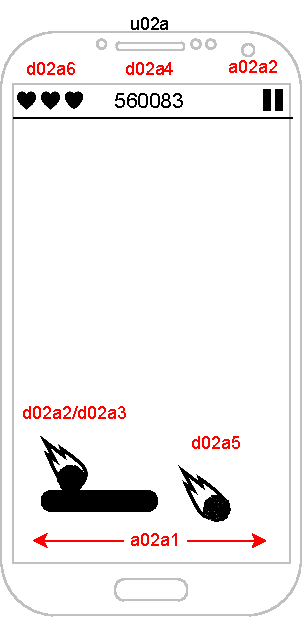
\includegraphics[scale=1.4]{diagramme/pdf/Mockup-u02a.pdf}
    \end{center}
    \caption{Dialog u02a - Spiel Classic}\label{fig:dia:u02a}
\end{figure}

Der Screen "Spiel Classic" muss neben dem beweglichen \gls{balken} (a02a1) und dem \gls{ball} die aktuelle Lebensanzeige und die aktuelle Punktzahl anzeigen.
Außerdem muss in der rechten oberen Ecke ein Pause-Button sein, welcher die Möglichkeit bietet, das aktuelle Spiel zu pausieren (a02a2).
Das Spiel muss mit den vorher definierten Parametern zur Schwierigkeitsstufe initialisiert werden und der Ball muss zu jedem Spielstart mittig des \glspl{balken} spawnen.
Verpasst der Spieler den Ball mit dem Balken und der Ball berührt den unteren Bildschirmrand, muss ein Leben abgezogen oder das Spiel beendet werden (d02a5).
(siehe Fig. \ref{fig:dia:u02a})
\vspace*{1cm}
\clearpage

\subsubsection{Dialog u02b - Spiel Invasion}\label{dialog:invasion}

\begin{figure}[h!]
    \begin{center}
    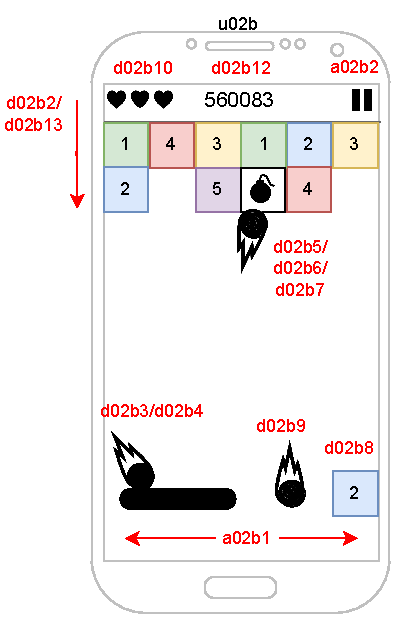
\includegraphics[scale=1.4]{diagramme/pdf/Mockup-u02b.pdf}
    \end{center}
    \caption{Dialog u02b - Spiel Invasion}\label{fig:dia:u02b}
\end{figure}

Bei dem optionalen Spielmodus \gls{invasionMode} können neben den UI-Elementen aus Dialog u02a noch die Spielmodus spezifischen Elemente auftauchen. 
Hierbei handelt es sich um Blöcke, welche zerstört werden können. Hierbei können die Blöcke unterschiedliche Stärken besitzen. 
Die Stärke repräsentiert die Anzahl an \gls{ball}berührungen, die es benötigt um einen Block zu zerstören. Außerdem können Power-Up Blöcke
erscheinen, welche dem \gls{spieler} temporäre Vorteile verschaffen können. Berührt ein Block den unteren Rand des Bildschirms, so muss das Spiel ebenfalls beendet werden (d02b8).
Wie bei dem \gls{classicMode}, muss auch hier das Spiel pausiert oder frühzeitig beendet werden können und mit der zuvor ausgewählten Schwierigkeitsstufe (leicht, mittel, schwer) initialisiert werden. Der Ball muss zu jedem Spielstart mittig des \glspl{balken} spawnen.
(siehe Fig. \ref{fig:dia:u02b})
\clearpage

\subsubsection{Dialog u09 - Sprachauswahl}\label{dialog:Sprachauswahl}

\begin{figure}[h!]
    \begin{center}
    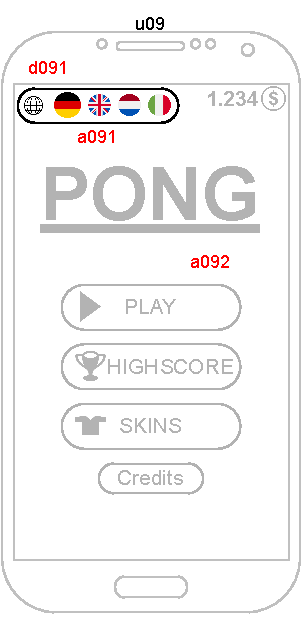
\includegraphics[scale=1.4]{diagramme/pdf/Mockup-u09.pdf}
    \end{center}
    \caption{Dialog u09 - Sprachauswahl}\label{fig:dia:u09}
\end{figure}

Bei der optionalen Sprachauswahl kann der \gls{spieler} zwischen verschiedenen Sprachen wählen und somit den im Spiel angezeigten Text entsprechend der Auswahl übersetzen lassen.
Die Flaggen repräsentieren hierbei die jeweilige Landessprache. Während der Sprachauswahl muss der Hintergrund ausgegraut sein und durch einen Klick ausserhalb des Sprachauswahl-Bereichs wieder verlassen werden können.
(siehe Fig. \ref{fig:dia:u09})
\clearpage

\subsubsection{Dialog u10 - Pause-Menü}\label{dialog:pause}

\begin{figure}[h!]
    \begin{center}
    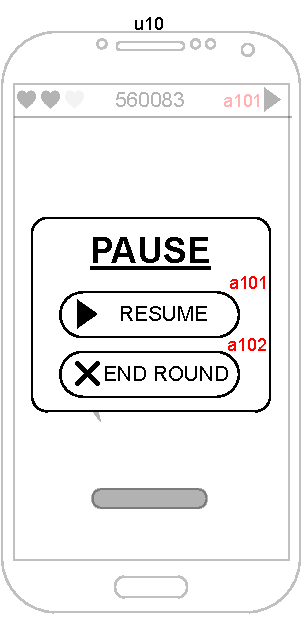
\includegraphics[scale=1.4]{diagramme/pdf/Mockup-u10.pdf}
    \end{center}
    \caption{Dialog u10 - Pause-Menü}\label{fig:dia:u10}
\end{figure}

Das Pause-Menü ist als ein Overlay über dem pausierten Spiel gestaltet und muss dem \gls{spieler} die Optionen geben, entweder das Spiel zu beenden (a102) oder das Spiel fortzusetzen (a101).
Der Hintergrund muss hierbei ausgegraut dargestellt werden.
(siehe Fig. \ref{fig:dia:u10})

\clearpage

\subsubsection{Dialog u11 - Game-Over-Menü} \label{subsec:u11-gameOverMenu}

\begin{figure}[h!]
    \begin{center}
    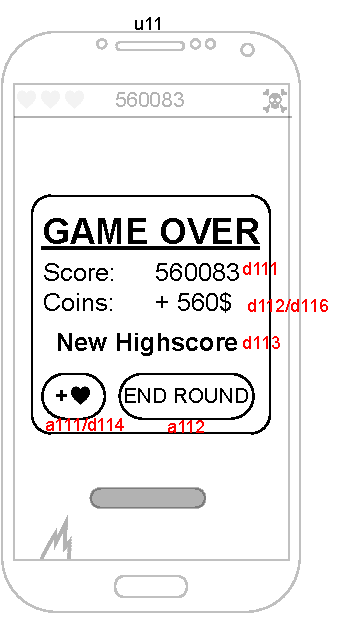
\includegraphics[scale=1.4]{diagramme/pdf/Mockup-u11.pdf}
    \end{center}
    \caption{Dialog u11 - Game-Over-Menü}\label{fig:dia:u11}
\end{figure}

Hat der \gls{spieler} keine Leben mehr, so muss der Game-Over Screen als Overlay angezeigt werden. Dieser muss dem Spieler beim ersten Mal nach jeder Spielrunde die Möglichkeit bieten eine letzte Chance zu bekommen (a111).
Diese letzte Chance muss sich durch einen Klick auf den Herz-Button auslösen lassen.
Außerdem müssen der erreichte Score (d111) und die erspielten Coins (d112) angezeigt werden.
Der \gls{spieler} muss mit einem Klick auf "End Round" (a112) zurück ins Hauptmenü geleitet werden.
Der Hintergrund muss hierbei ausgegraut dargestellt werden. 
(siehe Fig. \ref{fig:dia:u11})
\clearpage

\subsubsection{Dialog u12 - Werbung}\label{dialog:Werbung}

\begin{figure}[h!]
    \begin{center}
    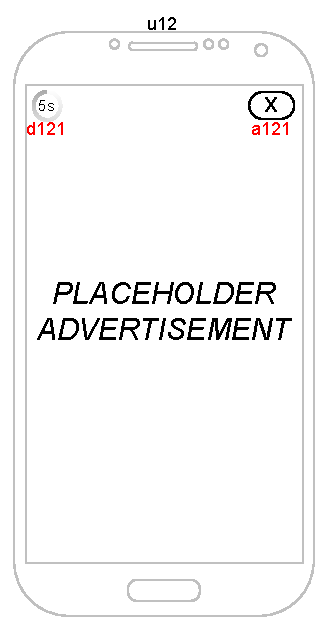
\includegraphics[scale=1.4]{diagramme/pdf/Mockup-u12.pdf}
    \end{center}
    \caption{Dialog u12 - Werbung}\label{fig:dia:u12}
\end{figure}


Entscheidet sich der \gls{spieler} dazu, Werbung anzuschauen um ein weiteres Leben zu bekommen, so wird ihm ein Werbeclip angezeigt.
Nach Ablauf der Werbung muss der \gls{spieler} diese durch einen Klick auf den X-Button beenden können (a121).
Woraufhin das Spiel mit einem letzten Leben fortgesetzt werden muss. Falls der Spieler im \gls{invasionMode} keine \gls{leben} mehr hat, muss das Spiel nach Ablauf der Werbung neu initialisiert werden. Entscheidet sich der \gls{spieler} vorzeitig dazu, dass er 
die Werbung nicht weiter schauen möchte, so muss er diese vorher beenden und somit auch den gesamten Spiel-Durchlauf beenden können (a121).
(siehe Fig. \ref{fig:dia:u12})
\clearpage

\subsubsection{Dialog u13 - Namenseingabe}\label{dialog:Namenseingabe}

\begin{figure}[h!]
    \begin{center}
    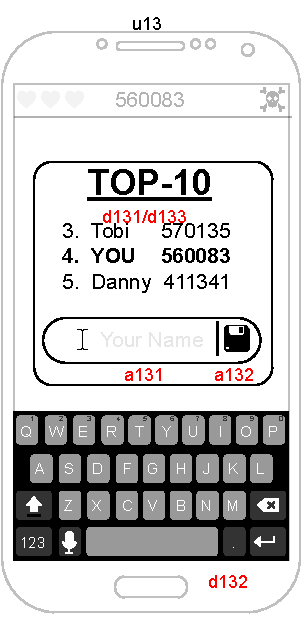
\includegraphics[scale=1.4]{diagramme/pdf/Mockup-u13.pdf}
    \end{center}
    \caption{Dialog u13 - Namenseingabe}\label{fig:dia:u13}
\end{figure}

Hat der \gls{spieler} eine \gls{Top10} Platzierung erspielt, so muss ihm seine Position in der \gls{Top10} Liste nach Ablauf der Spielrunde angezeigt werden.
Neben dem gerade erspielten Score müssen ebenfalls die zwei nächsten Scores angezeigt werden.
Der \gls{spieler} muss die Möglichkeit haben, seinen Namen einzutragen (a131) und sich mit einem Klick auf den Speichern-Button (a132) in der \gls{Top10} Liste abzuspeichern.
(siehe Fig. \ref{fig:dia:u13})
\clearpage

\subsubsection{Dialog u20 - Top-10 Liste}\label{dialog:top10}

\begin{figure}[h!]
    \begin{center}
    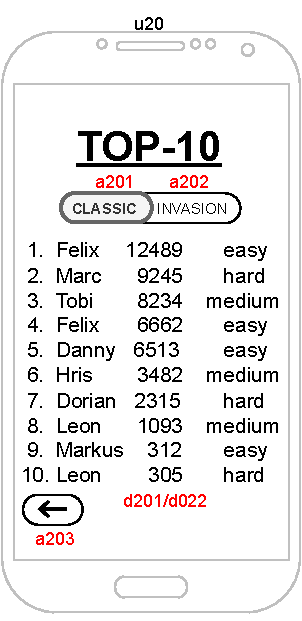
\includegraphics[scale=1.4]{diagramme/pdf/Mockup-u20.pdf}
    \end{center}
    \caption{Dialog u20 - Top-10 Liste}\label{fig:dia:u20}
\end{figure}

Die \gls{Top10} Liste muss die zehn besten Scores zeigen. Es kann für jeden Spielmodus eine einzelne Liste geben (\gls{invasionMode}, \gls{classicMode}). 
Es müssen Platzierung, Name des \glspl{spieler}, erreichte Punkte und Schwierigkeitsgrad angezeigt werden. Es soll ebenfalls die Möglichkeit geben, zwischen den \gls{Top10} Listen der jeweiligen Spielmodi wechseln zu können.
Durch einen Klick auf den Zurück-Button muss es möglich sein, zurück ins Hauptmenü zu gelangen.
(siehe Fig. \ref{fig:dia:u20})
\clearpage

\subsubsection{Dialog u25 - Achievements}\label{dialog:Achievements}

\begin{figure}[h!]
    \begin{center}
        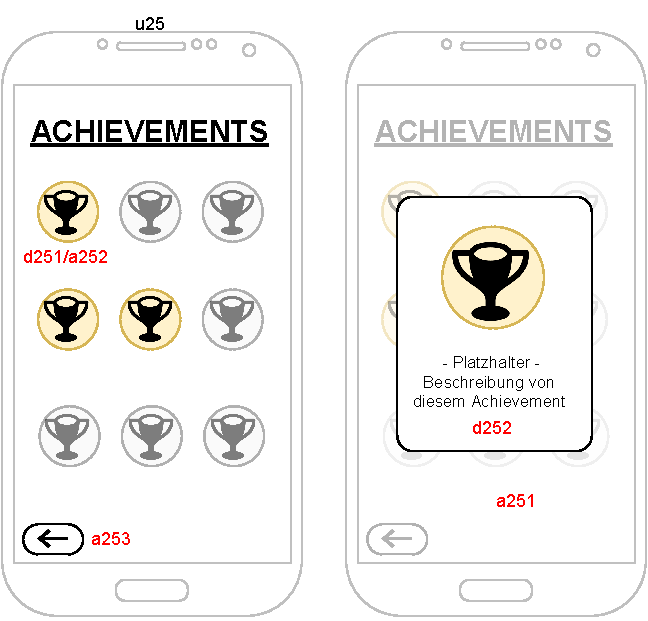
\includegraphics[scale=1.4]{diagramme/pdf/Mockup-u25.pdf}
    \end{center}
    \caption{Dialog u25 - Achievements}\label{fig:dia:u25}
\end{figure}

Auf dem Achievements Bildschirm können alle erreichbaren \gls{achievements} als Symbol dargestellt werden. Noch nicht freigeschaltete \gls{achievements} können hier ausgegraut dargestellt werden. Klickt der \gls{spieler} auf ein Achievementsymbol, kann die dazugehörige Beschreibung angezeigt werden. Ein Klick außerhalb der Beschreibung sorgt dafür, dass diese sich wieder schließt.
Dem \gls{spieler} kann es möglich sein, durch einen Klick auf den Zurück-Button wieder ins Hauptmenü zu gelangen.
(siehe Fig. \ref{fig:dia:u25})
\clearpage

\subsubsection{Dialog u30 - Skin-Auswahl}\label{dialog:skins}

\begin{figure}[h!]
    \begin{center}
    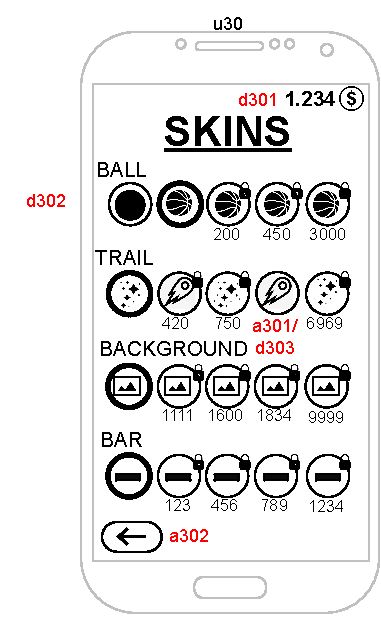
\includegraphics[scale=1.4]{diagramme/pdf/Mockup-u30.pdf}
    \end{center}
    \caption{Dialog u30 - Skin-Auswahl}\label{fig:dia:u30}
\end{figure}

Die Skin-Auswahl muss dem \gls{spieler} fünf Skins bieten, jeweils für den \gls{ball}, den Schweif, den Hintergrund und den \gls{balken}.
Dem \gls{spieler} muss es möglich sein, durch einen Klick auf den Zurück-Button wieder ins Hauptmenü zu gelangen.
Außerdem muss der \gls{spieler} sein aktuelles \gls{coin}-Guthaben in der rechten oberen Ecke angezeigt bekommen.
(siehe Fig. \ref{fig:dia:u30})
\clearpage

\subsubsection{Dialog u31 - Skin-Kauf}\label{dialog:skinkauf}

\begin{figure}[h!]
    \begin{center}
    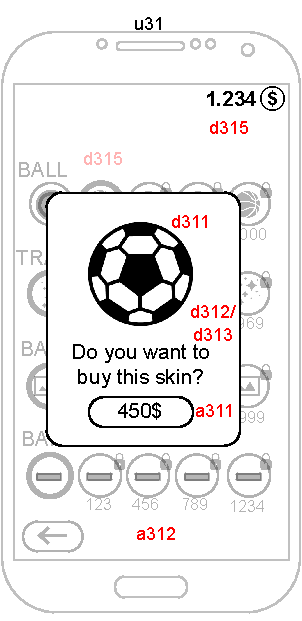
\includegraphics[scale=1.4]{diagramme/pdf/Mockup-u31.pdf}
    \end{center}
    \caption{Dialog u31 - Skin-Kauf}\label{fig:dia:u31}
\end{figure}

Kauft der \gls{spieler} einen Skin, so muss der Skin in einem Overlay vergrößert angezeigt werden. Außerdem muss der Preis angezeigt werden.
Der Hintergrund muss ausgegraut dargestellt werden und der \gls{spieler} muss sein aktuelles \gls{coin}-Guthaben in der rechten oberen Ecke angezeigt bekommen.
(siehe Fig. \ref{fig:dia:u31})
\clearpage

\subsubsection{Dialog u40 - Credits}\label{dialog:credits}

\begin{figure}[h!]
    \begin{center}
    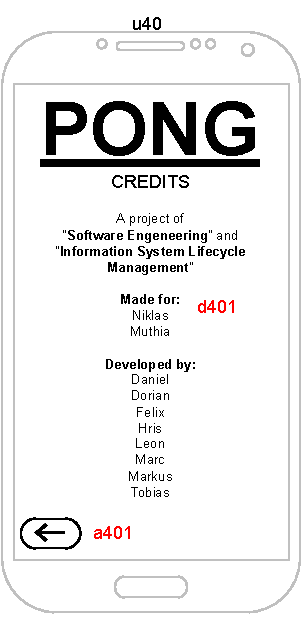
\includegraphics[scale=1.4]{diagramme/pdf/Mockup-u40.pdf}
    \end{center}
    \caption{Dialog u40 - Credits}\label{fig:dia:u40}
\end{figure}

Der \gls{spieler} muss die Möglichkeit haben in den Credits genauere Informationen zum Entwicklerteam und zur App allgemein zu bekommen.
Durch einen Klick auf den Zurück-Button, muss der \gls{spieler} wieder ins Hauptmenü gelangen.
(siehe Fig. \ref{fig:dia:u40})
\clearpage

    \clearpage

    \section{Produktdaten}\label{sec:produktdaten}
        \subsection{Mengengerüste}
    \subsubsection{Netzwerk}
    Das Spiel \gls{muss} einen Einzelspielermodus besitzen und offline spielbar sein. Es wird auf sämtliche Mehrspieler- sowie Netzwerk-Funktionen (ausschließlich Werbung) verzichtet.
    \subsubsection{Laufzeit}
    Ein Spieldurchlauf auf der Schwierigkeit "Medium" \gls{muss} ca. fünf Minuten beanspruchen. Das Abstimmen der Laufzeit für die Schwierigkeiten "Easy" und "Hard" ist dem Entwicklerteam überlassen.
\\
Die App darf nicht während eines Spieldurchlaufs abstürzen. Nach dem Drücken des Play-Buttons \gls{sollte} der Spieldurchlauf innerhalb von 5 Sekunden laden.
    \subsubsection{Display}
    Die Darstellung \gls{muss} entsprechend der Bildschirmgröße automatisch skaliert werden und lediglich im Hochkant-Modus des Endgeräts erfolgen.
Das Spielinterface \gls{muss} außerdem dunkel stilisiert sein und helle Akzente aufweisen.
    \subsubsection{Sound}
    Es ist zwar nicht für den Endprodukt erforderlich, dass das Spiel einen Ton abspielt, \gls{sollte} aber in angemessenen Situationen Sound wiedergeben.
    \subsubsection{Eingabe}
    Die Eingabe \gls{muss} durch den Touchscreen des Endgeräts erfolgen, auf dem das Spiel installiert ist.
Falls die Soundfunktion implementiert wurde, \gls{sollte} die Stärke des Geräusches im \hyperref[fig:dia:mainMenu]{Hauptmenü} und/oder durch das E/A des Betriebssystems gesteuert werden.
    \subsubsection{Einstellungen}
    Das Spiel \gls{muss} die Auswahl zwischen drei Schwierigkeitsstufen ("Easy", "Medium" und "Hard") erlauben.
Die App \gls{muss} die Möglichkeit bieten, den Skin für Ball, Schweif, Balken und Hintergrund anpassen zu können.\\
Die App \gls{sollte} eine Auswahl für den Spielmodus (\hyperref[fig:dia:classic]{Classic}/\hyperref[fig:dia:invasion]{Invasion}) bieten.
Außerdem \gls{sollte} eine Sprachauswahl eingebaut sein.

\clearpage
\subsection{Vorgaben Hardware und Software}
    \subsubsection{Hardware}
    \begin{wrapfigure}[8]{l}{0.5\textwidth}
    \begin{xltabular}{0.5\textwidth}{l r}
        \hline
        \textbf{Komponente} & \textbf{Mindestanforderung}   \\ \hline
        CPU                 & Snapdragon 450                \\
        RAM                 & 2 GiB (2086 MiB)              \\
        \caption{Hardwareanforderungen}\label{tab:hardwareRequirements}
    \end{xltabular}
\end{wrapfigure}

Um Fehler und Abstürze des Spiels durch veraltete Hardware auszuschließen, werden die
folgenden Spezifikationen als \textbf{Mindestanforderungen} in Tabelle
\ref{tab:hardwareRequirements} vorausgesetzt. Äquivalente oder überlegene Modelle der
Komponenten werden somit garantiert unterstützt.

\vspace{12pt}

\textit{
    Die obigen Werte unterstehen den Implementierungswünschen nach aktuellen
    Requirements (siehe Kapitel \ref{sec:requirements}) und können sich bei nachträglichen
    Änderungswünschen und auch durch Balancing (siehe Kapitel \ref{subsec:balancing}) ändern.
}


    \subsubsection{Software}\label{subsubsec:softwareMinReq}
    Das Spiel \gls{muss} ausschließlich als App für das Betriebssystem Android entwickelt werden (Version - siehe Kapitel \ref{subsec:bedienbarkeit}). Die Auswahl der Programmiersprache und der Versionsanforderungen darf das Entwicklerteam treffen.

\subsection{Lieferumfang}\label{subsec:lieferumfang}
Bei Auslieferung der Applikation umfasst diese folgenden Rahmen:

\begin{enumerate}
    \item \texttt{.apk}-Datei, bereitgestellt über eine öffentliche URL
    \item Installationsanleitung je nach Gerätespezifikation (auf Anfrage)
\end{enumerate}

\clearpage

\subsection{Balancing}\label{subsec:balancing}
Einige Anforderungen lassen sich nicht genau spezifizieren und/oder können erst während der Entwicklung genauer festgelegt werden.
Dies umfasst unter anderem - aber nicht beschränkend auf - das Reaktionsverhalten und die Haptik der \gls{balken}-Steuerung,
die Gewichtung und Verteilung numerischer Attribute wie z.B. \gls{point}-Multiplikatoren je Schwierigkeitsgrad und einige Designs.

\vspace{1em}

Diese Variablen werden absichtlich nicht in diesem Lastenheft aufgeführt, da die letztendliche Festsetzung dieser Parameter
"auf gut Glück" das Design der Applikation auf eine festgelegte Richtung setzt, von der zum aktuellen Stand nicht
absehbar ist, ob sie dem Auftraggeber gefällt.

\vspace{1em}

Die Parteien einigen sich auf eine offene Formulierung dieser Anforderungen, wie in Kapitel \ref{sec:requirements} und
ein Balancing im Laufe der Spielentwicklung. Der Auftraggeber erhält durch die \gls{beta} die Möglichkeit, weitere Änderungswünsche
bezüglich dieser Parameter zu äußern.

Die maximale Anzahl an Änderungsiterationen zwischen \gls{beta} und \gls{release} wird hiermit auf 3 beschränkt.

    \clearpage

    \section{Produktleistung, Performance}\label{sec:performance}
        Die App \gls{muss} alle Funktionen des Spiels in angemessener Zeit durchführen. 
Während des Spiels \gls{muss} es die Möglichkeit zur Pausierung geben.
Die Framerate ist von der Hardware abhängig und kann somit nicht garantiert werden.
Nach einem Neustart der App müssen alle Highscores, \glspl{skin} und Einstellungen gespeichert bleiben. 
    \clearpage

    \section{Qualitätsanforderungen}\label{sec:quality}
        \subsection{Bedienbarkeit \& Zuverlässigkeit \& Effizienz}\label{subsec:bedienbarkeit}
        Das Spiel PONG \gls{muss} auf allen Mobilgeräten mit den in Kapitel \ref{subsubsec:softwareMinReq}
beschriebenen Mindestanforderungen fehlerfrei laufen und bedienbar sein.

Dabei gilt, dass das Endgerät mindestens mit Android 10 laufen \gls{muss},
um versionsbedingte Fehler zu vermeiden. Des Weiteren \gls{muss} sichergestellt werden,
dass keine Fehler auftreten, die vom Programmcode des Spiels ausgehen.


        \subsection{Anforderungen an die Änderbarkeit}
        Bei der Entwicklung der Software für das Spiel PONG \gls{muss} sich an gängige Konventionen gehalten werden, um zu gewährleisten, dass das Ändern oder Hinzufügen von Programmcode möglichst einfach stattfinden kann. 

        \subsection{Anforderungen an die Darstellung}
        Das Spiel wird im Hochkant Format ausgeführt und \gls{muss} abhängig von der Bildschirmgröße passend skaliert sein. 

        \subsection{Testbarkeit}\label{subsec:tests}
        Im Laufe der Entwicklung wird es Tests geben, welche nur teilweise automatisch realisiert werden können.
Die Anforderungen an die App machen es nicht möglich, die gesamten Funktionalitäten automatisch testen zu lassen.
Daher wird es während des Entwicklungsprozesses ausführliche, händische Tests geben, um die Bedienbarkeit und das Spielgefühl zu testen.

    \clearpage

    \section{Tabellarische Requirements}\label{sec:requirements}
        \subsection{Mengengerüste}
    \subsubsection{Netzwerk}
    Das Spiel \gls{muss} einen Einzelspielermodus besitzen und offline spielbar sein. Es wird auf sämtliche Mehrspieler- sowie Netzwerk-Funktionen (ausschließlich Werbung) verzichtet.
    \subsubsection{Laufzeit}
    Ein Spieldurchlauf auf der Schwierigkeit "Medium" \gls{muss} ca. fünf Minuten beanspruchen. Das Abstimmen der Laufzeit für die Schwierigkeiten "Easy" und "Hard" ist dem Entwicklerteam überlassen.
\\
Die App darf nicht während eines Spieldurchlaufs abstürzen. Nach dem Drücken des Play-Buttons \gls{sollte} der Spieldurchlauf innerhalb von 5 Sekunden laden.
    \subsubsection{Display}
    Die Darstellung \gls{muss} entsprechend der Bildschirmgröße automatisch skaliert werden und lediglich im Hochkant-Modus des Endgeräts erfolgen.
Das Spielinterface \gls{muss} außerdem dunkel stilisiert sein und helle Akzente aufweisen.
    \subsubsection{Sound}
    Es ist zwar nicht für den Endprodukt erforderlich, dass das Spiel einen Ton abspielt, \gls{sollte} aber in angemessenen Situationen Sound wiedergeben.
    \subsubsection{Eingabe}
    Die Eingabe \gls{muss} durch den Touchscreen des Endgeräts erfolgen, auf dem das Spiel installiert ist.
Falls die Soundfunktion implementiert wurde, \gls{sollte} die Stärke des Geräusches im \hyperref[fig:dia:mainMenu]{Hauptmenü} und/oder durch das E/A des Betriebssystems gesteuert werden.
    \subsubsection{Einstellungen}
    Das Spiel \gls{muss} die Auswahl zwischen drei Schwierigkeitsstufen ("Easy", "Medium" und "Hard") erlauben.
Die App \gls{muss} die Möglichkeit bieten, den Skin für Ball, Schweif, Balken und Hintergrund anpassen zu können.\\
Die App \gls{sollte} eine Auswahl für den Spielmodus (\hyperref[fig:dia:classic]{Classic}/\hyperref[fig:dia:invasion]{Invasion}) bieten.
Außerdem \gls{sollte} eine Sprachauswahl eingebaut sein.

\clearpage
\subsection{Vorgaben Hardware und Software}
    \subsubsection{Hardware}
    \begin{wrapfigure}[8]{l}{0.5\textwidth}
    \begin{xltabular}{0.5\textwidth}{l r}
        \hline
        \textbf{Komponente} & \textbf{Mindestanforderung}   \\ \hline
        CPU                 & Snapdragon 450                \\
        RAM                 & 2 GiB (2086 MiB)              \\
        \caption{Hardwareanforderungen}\label{tab:hardwareRequirements}
    \end{xltabular}
\end{wrapfigure}

Um Fehler und Abstürze des Spiels durch veraltete Hardware auszuschließen, werden die
folgenden Spezifikationen als \textbf{Mindestanforderungen} in Tabelle
\ref{tab:hardwareRequirements} vorausgesetzt. Äquivalente oder überlegene Modelle der
Komponenten werden somit garantiert unterstützt.

\vspace{12pt}

\textit{
    Die obigen Werte unterstehen den Implementierungswünschen nach aktuellen
    Requirements (siehe Kapitel \ref{sec:requirements}) und können sich bei nachträglichen
    Änderungswünschen und auch durch Balancing (siehe Kapitel \ref{subsec:balancing}) ändern.
}


    \subsubsection{Software}\label{subsubsec:softwareMinReq}
    Das Spiel \gls{muss} ausschließlich als App für das Betriebssystem Android entwickelt werden (Version - siehe Kapitel \ref{subsec:bedienbarkeit}). Die Auswahl der Programmiersprache und der Versionsanforderungen darf das Entwicklerteam treffen.

\subsection{Lieferumfang}\label{subsec:lieferumfang}
Bei Auslieferung der Applikation umfasst diese folgenden Rahmen:

\begin{enumerate}
    \item \texttt{.apk}-Datei, bereitgestellt über eine öffentliche URL
    \item Installationsanleitung je nach Gerätespezifikation (auf Anfrage)
\end{enumerate}

\clearpage

\subsection{Balancing}\label{subsec:balancing}
Einige Anforderungen lassen sich nicht genau spezifizieren und/oder können erst während der Entwicklung genauer festgelegt werden.
Dies umfasst unter anderem - aber nicht beschränkend auf - das Reaktionsverhalten und die Haptik der \gls{balken}-Steuerung,
die Gewichtung und Verteilung numerischer Attribute wie z.B. \gls{point}-Multiplikatoren je Schwierigkeitsgrad und einige Designs.

\vspace{1em}

Diese Variablen werden absichtlich nicht in diesem Lastenheft aufgeführt, da die letztendliche Festsetzung dieser Parameter
"auf gut Glück" das Design der Applikation auf eine festgelegte Richtung setzt, von der zum aktuellen Stand nicht
absehbar ist, ob sie dem Auftraggeber gefällt.

\vspace{1em}

Die Parteien einigen sich auf eine offene Formulierung dieser Anforderungen, wie in Kapitel \ref{sec:requirements} und
ein Balancing im Laufe der Spielentwicklung. Der Auftraggeber erhält durch die \gls{beta} die Möglichkeit, weitere Änderungswünsche
bezüglich dieser Parameter zu äußern.

Die maximale Anzahl an Änderungsiterationen zwischen \gls{beta} und \gls{release} wird hiermit auf 3 beschränkt.

    \clearpage

    \section*{Lastenheftabnahme}
    \addcontentsline{toc}{section}{\protect\numberline{}Lastenheftabnahme}
        Durch meine Unterschrift bestätige ich, dass das vorliegende Lastenheft in seinem Umfang
und in seiner Ausführung den getroffenen Vereinbarungen zwischen Auftraggeber und
Auftragnehmer entspricht und dass dieses Lastenheft für Auftraggeber und Auftragnehmer
eine verbindliche Projektgrundlage bildet.

\vspace{1em}

Änderungswünsche, die dem Auftraggeber in diesem Lastenheft ausdrücklich zugesichert werden
sind weiterhin gültig, siehe Kapitel \ref{subsec:lieferumfang}, \ref{subsec:balancing}, \ref{subsec:tests}.

\vspace{2cm}

\begin{xltabular}{\textwidth}{XXX}
    \dotfill            & \dotfill                  & \dotfill              \\
    \textit{Ort, Datum} & \textit{Auftragnehmer}    & \textit{Auftraggeber} \\
\end{xltabular}

    \clearpage

    \gdef\listfigurename{Abbildungsverzeichnis}
    \addcontentsline{toc}{section}{\listfigurename}
    \listoffigures
    \clearpage
    \gdef\listtablename{Tabellenverzeichnis}
    \addcontentsline{toc}{section}{\listtablename}
    \listoftables
    \clearpage

    \printglossary[title=Glossar, toctitle=Glossar]
    % \clearpage

\end{document}
